\section{Polyadic Quantification Theory}

\subsection{Introduction to PQT}
It's now time to turn to the final logic we will study, Polyadic Quantification Theory\footnote{Also called \emph{First Order Logic}}, which allows predicates of arbitrary arity as opposed to just monadic predicates like in MQT. Although it is a straightforward extension of MQT, we will see that allowing relations of any arity changes the properties of the logic substantially. 

As opposed to truth-functional and monadic logic which, as we've seen, are of limited expressive power, polyadic quantification theory allows for faithful schematization of vast tracts of scientific discourse. For an example, we begin not with science, but with literature.

Consider the sentences
\begin{itemize}
\item
Romeo loves Juliet.
\item
Someone loves Juliet.
\item
Romeo loves someone.
\end{itemize}
The first sentence implies the second and the third sentence.
We can schematize the second, by making use of the monadic predicate ``$\bigcirc\ \mathrm{loves\ Juliet}$'' thus
\[(\exists x)(x\ \mathrm{loves\ Juliet}).\]
And we can schematize the third, by making use of the monadic predicate ``$\mathrm{Romeo\ loves}\ \bigcirc$'' thus
\[(\exists x)(\mathrm{Romeo\ loves}\ x).\]
But if we wish to schematize the sentence ``someone loves someone,'' which is also implied by the first sentence above, we need to expand our resources to include \emph{dyadic predicates} - ie, predicates which act on \emph{ordered pairs}, not just single elements (like monadic predicates).
\begin{itemize}
\item
$\fbox{1}\ \mathrm{loves}\ \fbox{2}$
\item
$\langle \mathrm{Romeo,Juliet} \rangle$ is in the extension of 
``$\fbox{1}\ \mathrm{loves}\ \fbox{2}$.''
\item
$(\exists x)(\exists y)(x\ \mathrm{loves}\ y)$
\end{itemize}

The extension of a dyadic predicate is a set of \emph{ordered} pairs.
\begin{itemize}
\item
$\langle 45,47 \rangle$ is in the extension of ``$\fbox{1} \leq \fbox{2}$.''
\item
$\langle 45,47 \rangle$ is not in the extension of ``$\fbox{2} \leq \fbox{1}$.''
\item
$\langle 47,45 \rangle$ is in the extension of ``$\fbox{2} \leq \fbox{1}$.''
\end{itemize}

Similarly, the extension of a triadic predicate, such as 
\begin{quote}
``$\fbox{1}\ \mathrm{is\
further\ from}\ \fbox{2}\ \mathrm{than\ it\ is\ from}\ \fbox{3}$,'' 
\end{quote}
is a set of
ordered triples.

Evidently, this idea generalizes to all dimensions $n \leq 1$; not only just the $2$-variable ordered paris and the $3$-variable ordered triplets. In general, an $n$-ary predicate on a universe $U$ is any subset of the \emph{Cartesian Product} $U^n$, ie the set of tuples of length $n$ whose components are in $U$. 

For simplicity's sake, we will normally confine ourselves to the binary and ternary cases in examples and exposition. 
\newpage



\subsection*{Quantifier alternation}
Consider the following statements involving alternation of quantifiers.
\begin{itemize}
\item
Everyone loves someone (or other).
\[S_1:\ \ \ (\forall x)(\exists y)(x\ \mathrm{loves}\ y).\]
\item
There is someone whom everyone loves.
\[S_2:\ \ \ (\exists y)(\forall x)(x\ \mathrm{loves}\ y).\]
\item
Everyone is loved by someone (or other).
\[S_3:\ \ \ (\forall y)(\exists x)(x\ \mathrm{loves}\ y).\]
\item
There is someone who loves everyone.
\[S_4:\ \ \ (\exists x)(\forall y)(x\ \mathrm{loves}\ y).\]
\end{itemize}
The second statement implies the first, and the fourth implies the third. 
%None of these statements means something different (ie none are equivalent) - and so we see immediately that \emph{the order in which quantifiers appear matters}. 
\begin{aside}
    Give an intuitive argument to show %, although no two of the above statements are equivalent, 
    that $S_2$ implies $S_1$, and that $S_4$ implies $S_3$. 
\end{aside}

%Aside from the implications $S_2 \implies S_1$ and $S_4 \implies S_3$, no other implications hold. To see this, 
In order to show that no other implications hold,
we introduce schemata to represent the statements $S_1,\ldots,S_4$, and the notion of a structure suitable for their interpretation.

\subsection*{Schemata and Structures}

Just as we did in the case of truth-functional logic and monadic quantification theory, we introduce a formal language for schematizing statements involving polyadic predicates. The only change to the vocabulary of monadic quantification theory is the addition of polyadic predicate letters. For example, we introduce dyadic predicate letters such as $L\ \fbox{1}\ \fbox{2}$ to schematize dyadic predicates such as $\fbox{1}$ loves $\fbox{2}$ or $\fbox{1}\leq \fbox{2}$.
We may then use this dyadic predicate letter to schematize the four statements above as follows.
\begin{itemize}
\item $S_1:\ \ \ (\forall x)(\exists y)(Lxy)$
\item $S_2:\ \ \ (\exists y)(\forall x)(Lxy)$
\item $S_3:\ \ \ (\forall y)(\exists x)(Lxy)$
\item $S_4:\ \ \ (\exists x)(\forall y)(Lxy)$
\end{itemize}

We now extend the notion of a structure to the case of polyadic quantification theory. Again, a structure $A$ is determined by the specification of a nonempty set $U^A$, the universe of discourse of $A$, over which the variables of quantification range, and specifications of extensions of the polyadic predicates which appear in schemata that the structure will be used to interpret. Thus, in the case to hand, the specification of $A$ will require assigning to the dyadic predicate letter $L$, a set $L^A$ of ordered pairs of elements from $U^A$ as its extension. That is, $L^A\subseteq U^A\times U^A$, where $U^A\times U^A$ is the \emph{Cartesian product} of $U^A$ with itself -- the set $\{\op{a}{b}\mid a,b\in U^A\}$. 

The interpretation of the logical vocabulary, that is, truth-functional connectives and quantifiers, is the same in both monadic and polyadic quantification theory. Thus, we may introduce without further ado the notion of a schema $S$ of polyadic quantification being true in (or satisfied by) a structure $A$ that assigns extensions to all the polyadic predicate letters appearing in $S$ (written $A\models S$). If $S$ contains free variables, we must of course supplement the structure $S$ with assignments of elements from $U^A$ to those free variables. For example, we write
\[A\models S[(x|a)(y|b)]\]
for ``the structure $A$ satisfies the schema $S$ with respect to the assignments of $a$ to $x$ and $b$ to $y$.'' This notation is used with the understanding that no variables other than $x$ and $y$ occur free in $S$ and that $a,b\in U^A$. With this definition of satisfaction, our definitions of satisfiability, validity, implication, and equivalence for closed monadic quantificational schemata generalize immediately to PQT. For ease of reference, we restate them as follows.
\begin{itemize}
\item
A polyadic schema $S$ is \emph{ valid} if and only if for every structure $A, A
\models S.$
\item
A polyadic schema $S$ is \emph{ satisiable} if and only if for some structure $A,
A \models S.$
\item
A polyadic schema $S$ \emph{ implies} a polyadic schema $T$ if and only if for
every structure $A,$ if $A \models S,$ then $A \models T.$
\item
polyadic schemata $S$ and $T$ are equivalent if and only if $S$ implies $T$, and $T$ implies $S$. 
\end{itemize}
Thus, in order to show that a schema $S$ fails to imply a schema $T$, it suffices to exhibit a \emph{counterexample} to the implication, that is, a structure $A$ such that $A\models S$ and $A\not\models T$. We proceed to illustrate this technique by show that among the four schemata $S_1,\ldots,S_4$ discussed above, if $i\neq j$, then $S_i$ does not imply $S_j$ except in case $i=2$ and $j=1$, or $i=3$ and $j=4$.

We begin by specifying three structures $A,B,C$ which act as a counterexamples to various of these implications. First we let $U^A=U^B=U^C=\{1,2\}$. We specify the extension of $L$ in each structure as follows.%Consider the following three structures $A, B, C$.
\begin{itemize}
\item $L^A=\{\op{1}{1},\op{2}{2}\}.$
\item $L^B=\{\op{2}{2},\op{1}{2}\}.$
\item $L^C=\{\op{2}{2},\op{2}{1}\}.$
\end{itemize} 
\iffalse
\[
\begin{array}{| c | c | c |}
\hline
 \mbox{Structure}& \mbox{Universe} & \mbox{Extension of }L\\
  \hline            
  A & \{a,b\} & \{\op{a}{a},\op{b}{b}\}\\
  \hline
  B & \{a,b\} & \{\op{b}{b},\op{a}{b}\}\\
 \hline
 C & \{a,b\} & \{\op{b}{b},\op{b}{a}\}\\
 \hline  
\end{array}
\]
\fi
Note that $A\models S_1$ and $A\models S_3$, while $A\not\models S_2$ and $A\not\models S_4$, from which it follows, by definition, that $S_1$ does not imply $S_2$, nor does $S_3$ imply $S_4$. Moreover $B\models S_2$, but $B\not\models S_3$, and $C\models S_4$, but $C\not\models S_1$; thus $S_2$ does not imply $S_3$, and $S_4$ does not imply $S_1$. 

Failure of the remaining %(non-trivial) 
implications now follows. For example, $S_1$ does not imply $S_4$. To see this, suppose, \emph{ad reductio}, that $S_1$ implies $S_4$. Then since $S_2$ implies $S_1$ and $S_4$ implies $S_3$, it follows, by the transitivity of implication, that $S_2$ implies $S_3$. But we have already seen that $S_2$ does not imply $S_3$ ($B$ was the counterexample), a contradiction.

\begin{aside}
    Verify that each of the statements above is true. For example, if we claimed that $A \models S_i$ for some $i$, explain in your own words why, in fact, $A$ actually models $S_i$.  

    Show that the remaining non-trivial implications also fail. To do this, use proof-by-contradiction as we did to show that $S_1$ does not imply $S_4$. 
\end{aside}

We summarize the results of this discussion in the following matrix $\langle a_{ij}\mid 1\leq i,j\leq 4\rangle$, where $a_{ij} = 1$ if and only if the schema in the $i$-th row implies the schema in the $j$-th column.
\[
\begin{array}{| c | c | c | c | c|}
\hline
 S_i\mbox{ implies }S_j& S_1 & S_2 & S_3 & S_4\\
  \hline            
  S_1 & 1 & 0 & 0 & 0\\
  \hline
  S_2  & 1 & 1 & 0 & 0\\
 \hline
 S_3 & 0 & 0 & 1 & 0\\
 \hline
 S_4 & 0 & 0 & 1 & 1\\
 \hline  
\end{array}
\]


\subsection*{Quantificational ambiguity}

We briefly explore ambiguities that can arise in natural language via the interaction of quantifiers. Consider the statement, 
\begin{equation}\label{lover}
\mbox{``everybody loves a lover.''} 
\end{equation}
Statement (\ref{lover}) involves such an ambiguity. We can bring this out by offering two schematizations, each of which corresponds to a natural reading of this statement. 
We may schematize ``$x$ is a lover,'' again using the dyadic predicate letter $L$, as $(\exists y)Lxy$.%\footnote{There are two main styles for how to write an element in a binary relation. Here, we are using $Lxy$ to indicate that the relation $L$ holds between $x$ and $y$; this could also be written as $xLy$. We choose the former. When the relation is more naturally written in the center we will do so - ie for the relation ``less than'', we will write $x < y$ rather than $<xy$}. 
Now, consider the following two schemata.
\[(\forall z)(\exists x)((\exists y)Lxy\wedge Lzx)\]
\[(\forall x)((\exists y)Lxy\supset (\forall z)Lzx)\]
The first schema corresponds to the reading ``everybody loves someone who is a lover,'' while the second corresponds to the reading ``if someone is a lover, then everybody loves her.''
\iffalse
There are two natural %\footnote{Well, there are infinitely many \emph{possible} 
readings of that sentence. There are only two \emph{reasonable} ones} readings of the sentence ``everybody loves a lover'': either we interpret it as ``everybody loves someone who is a lover'', and ``if someone is a lover, then everybody loves her''. Corresponding to these two interpretations, we have the respective schematizations:

\[(\forall z)(\exists x)((\exists y)Lxy\wedge Lzx)\footnote{A decent reading of this schematization is ``for every person $z$, there is a person $x$ such that $z$ loves $x$ and there is a $y$ that $x$ loves''.}\] 
and 
\[(\forall x)((\exists y)Lxy\supset (\forall z)Lzx)\]
\fi

We claim that a structure $A$ satisfies the second schema if and only if either $L^A$ is empty or $L^A=U^A\times U^A$, the cartesian product of the universe of $A$ with itself. 

\begin{aside}
    Give an intuitive argument to verify this claim. 
\end{aside}

On the other hand, if a structure $B$ satisfies the first schema, then $L^B$ is non-empty; moreover, if $B$ consists of a pair of requiting lovers at least one of whom is not a narcissist, $B$ satisfies the first, but not the second, schema. Thus, neither disambiguation of the original sentence implies the other.
\iffalse
\begin{aside}
    Give two different schematizations of the sentence ``all that glitters is not gold'', corresponding to two different interpretations of the scope of the negation ``not''. 
\end{aside}
\fi
\newpage

% \subsection{Binary Relations}
We will now discuss several important properties which can hold of binary relations. Letting $L$ be our binary relation, we have the following definitions. 

\begin{definition}
$L^A$ is \emph{reflexive} if and only if
\[A\models (\forall x)Lxx.\]
\end{definition}

\begin{definition}
$L^A$ is \emph{irreflexive} if and only if
\[A\models (\forall x)\neg Lxx.\]
\end{definition}

\begin{definition}
$L^A$ is \emph{symmetric} if and only if
\[A\models (\forall x)(\forall y)(Lxy\supset Lyx).\]
\end{definition}

\begin{definition}
$L^A$ is \emph{asymmetric} if and only if
\[A\models (\forall x)(\forall y)(Lxy\supset \neg Lyx).\]
\end{definition}

\begin{definition}
$L^A$ is \emph{transitive} if and only if
\[A\models (\forall x)(\forall y)(\forall z)(Lxy\supset (Lyz\supset Lxz)).\]
\end{definition}

\begin{definition}
$A$ is a \emph{simple graph} if and only if $L^A$ is irreflexive and symmetric.
\end{definition}

\subsection*{Identity}
A new logical dyadic predicate, identity, will  allows us to ``put the quant into quantification.''The identity relation ``$=$'' has a uniform interpretation over all structures $A$ namely $=^A$ is equal to $\{\op{a}{a}\mid a\in U^A\}$. Since the interpretation of the identity relation is uniform, we omit mention of it when we specify structures.\footnote{We call identity a \emph{logical} predicate (as opposed to your garden-variety, run-of-the-mill predicates) because of this uniform interpretation across all structures. It means the same thing regardless of which structure you're in, so it is of logical character}. 

\begin{aside}
    Identity is, of course, an equivalence relation. Prove this. 
\end{aside}

\subsection*{Numerical quantifiers}
By making use of the identity relation, we can introduce, for each integer $k\geq 1$, the quantifiers ``there are at least $k$ $x$'s such that $S(x)$'', ``there are at most $k$ $x$'s such that $S(x)$'', and ``there are exactly  $k$ $x$'s such that $S(x)$'' as follows.
\[
\begin{array}{ll}
(\exists^{k\leq}x)S(x):  & (\exists x_1)\ldots(\exists x_k)(\bigwedge_{1\leq i<j\leq k}x_i\neq x_j\wedge \bigwedge_{1\leq i\leq k}S(x_i))\\
(\exists^{\leq k}x)S(x): & \neg (\exists^{k+1\leq}x)S(x)\\
(\exists^{ = k}x)S(x): & (\exists^{\leq k}x)S(x)\wedge(\exists^{k\leq}x)S(x)
\end{array}
\]

\begin{aside}
    The crux of our proof of the Small Model Theorem for MQT was that realizing the same types corresponded to satisfying the same monadic sentences. Of course, realizing the same types does not mean that two structures satisfy the same sentences of PQT: the identity relation allows us to distinguish structures by \emph{counting} how many elements realize a given type. \emph{A priori}, this does not mean that decidability (which was a corollary of our SMT) fails for PQT - only that our particular proof of the SMT for MQT would fail for PQT. We will see more about the decidability of MQT in the future. 
\end{aside}

Let's use $\card{X}$ to denote the number of members of a set $X$ (you may have seen this notation before to mean ``absolute value''; its interpretation here is similar but distinct).    
In order to clarify the import of these  numerical quantifiers, we introduce the notion of the \emph{set defined by a one variable open schema $S(x)$ in a structure $A$} (written $S[A]$):
\[S[A]=\{a\in U^A\mid A\models S[x|a]\}.\] That is, $S[A]$ is the set of members of $U^A$ that satisfy $S(x)$ in $A$. Observe that $A\models(\exists^{k\leq}x)S(x)$ if and only if $k\leq\card{S[A]}$, and similarly for the other two newly introduced quantifiers. Our next goal is to use these quantifiers to define regular simple graphs.
% \newpage

% \subsection{Graphs}
Recall that a \emph{graph} is structure that interprets a single dyadic predicate letter ``$L$'' (these are sometimes also called directed graphs to emphasize that the edges have directionality). Unless otherwise stated, we will restrict our attention for the rest of the course to structures that are graphs; this restriction doesn't lose us much (all results we will derive are easily generalizable to structures with arbitrary relations) and it adds much tabgibility. A graph $A$ is \emph{simple} if and only if $L^A$ is both irreflexive and symmetric (ie the edges are undirected, and tehre are no ``self loops'' at any node). We introduced the abbreviation \sg\ for the conjunction of the schemata expressing irreflexivity and symmetry, which we abbreviated as \irr\ and \sym, respectively. For a structure $A$, $A \models \sg$ iff $A$ is a simple graph. 

Note that for any two nodes $a, b$ in a simple graph, there can be \emph{at most one} edge $\langle a, b \rangle$ because the edge relation is a binary relation and hence a set (which disregards multiplicity). In the following definitions, suppose that $A$ is a simple graph with $a \in U^A$ (ie, $a$ is a node in the graph $A$). 

\begin{definition}
The \emph{neighborhood of $a$ in $A$} is $\nbh{a}{A} := \{b\in U^A\mid \op{a}{b}\in L^A\}$ (the set of all neighbours of $a$, eg the set of all nodes which $a$ is connected to). 
\end{definition}

\begin{definition}
The \emph{degree of $a$ in $A$} is $\dg{a}{A} := \card{\{b\in U^A\mid \op{a}{b}\in L^A\}}$ (the number of neighbours of $a$, or equivalently the number of edges incident to $a$).
\end{definition}


\begin{definition}
A simple graph is \emph{$k$-regular} if and only if all nodes of the graph have degree $k$. We can schematize this condition, using the dyadic predicate $L$ for the edge relation, as
\[(\forall y)(\exists^{=k}x)Lyx.\]
\end{definition}

What do the collections of 1-regular and 2-regular simple graphs look like? Every 1-regular graph consists of a set of independent edges, and that a \emph{finite} 2-regular graph consists of a collection of independent simple cycles, that is, graphs that may be drawn in the plane as a disjoint finite collection of disjoint polygons. As well, the doubly-infinite simple chain is also 2-regular (think of the integers, where there is an edge $\langle a, b \rangle$ iff $a = b \pm 1$). Polygons and bi-infinite chains exhaust the possible connected components of 2-regular graphs.

\subsection*{Counting graphs}

Just as we did for truth-functional logic and MQT, we can also count satisfying structures to sentences of PQT. In particular, we will count graphs with a fixed universe of discourse. To that end, we have the following definition. 

\begin{definition}
We denote the set of simple graphs on $n$ nodes which satisfy a sentence $S$ by $\modn{S}{n}$, eg: \[\modn{S}{n}=\{A\mid A\models S\mbox{ and }U^A=\{1,\ldots,n\}\}.\] 
\end{definition}

Note that for every structure $A$, $A\models (\forall x)x=x$, thus  $\modn{(\forall x)x=x}{n}$ is the set of all graphs with universe of discourse $\{1,\ldots,n\}$. 

Let's count the number of graphs $A$ with $U^A=\{1,2,3,4\}$ (by the previous comment, this is of course equal to $\card{\modn{(\forall x)x=x}{4}}$). Any such graph is determined by choosing which of the sixteen possible edges from $i$ to $j$ to draw, where $1\leq i\leq 4$ and $1\leq j\leq 4$; that is, a graph with this universe of discourse is determined by 16 binary choices, so, by the product rule, there are $2^{16}$ such graphs. Analogous reasoning leads to the conclusion that there are $2^{n^2}$ graphs with universe of discourse $\{1,\ldots, n\}$ (because there are $n^2$ pairs of nodes, and hence $2^{n^2}$ possible edge-sets). Similarly, since a simple graph with universe of discourse $\{1,\ldots, n\}$ is determined by making a choice from a collection of $\binom{n}{2}$ possible \emph{undirected} edges, there are $2^{\binom{n}{2}}$ simple graphs $A$ with $U^A=\{1,\ldots, n\}$. 

\begin{aside}
    How many 1-regular simple graphs are there with universe of discourse $\{1,\ldots, n\}$? 
\end{aside}


% \newpage

\subsection{Binary Relations, Functions, and Graphs}
We will now discuss several important properties which can hold of binary relations. Letting $L$ be our binary relation, we have the following definitions. 

\begin{definition}
$L^A$ is \emph{reflexive} if and only if
\[A\models (\forall x)Lxx.\]
\end{definition}

\begin{definition}
$L^A$ is \emph{irreflexive} if and only if
\[A\models (\forall x)\neg Lxx.\]
\end{definition}

\begin{definition}
$L^A$ is \emph{symmetric} if and only if
\[A\models (\forall x)(\forall y)(Lxy\supset Lyx).\]
\end{definition}

\begin{definition}
$L^A$ is \emph{asymmetric} if and only if
\[A\models (\forall x)(\forall y)(Lxy\supset \neg Lyx).\]
\end{definition}

\begin{definition}
$L^A$ is \emph{transitive} if and only if
\[A\models (\forall x)(\forall y)(\forall z)(Lxy\supset (Lyz\supset Lxz)).\]
\end{definition}

\begin{definition}
$A$ is a \emph{simple graph} if and only if $L^A$ is irreflexive and symmetric.
\end{definition}

\subsection*{Identity}
A new logical dyadic predicate, identity, will  allows us to ``put the quant into quantification.''The identity relation ``$=$'' has a uniform interpretation over all structures $A$ namely $=^A$ is equal to $\{\op{a}{a}\mid a\in U^A\}$. Since the interpretation of the identity relation is uniform, we omit mention of it when we specify structures.\footnote{We call identity a \emph{logical} predicate (as opposed to your garden-variety, run-of-the-mill predicates) because of this uniform interpretation across all structures. It means the same thing regardless of which structure you're in, so it is of logical character}. 

\begin{aside}
    Identity is, of course, an equivalence relation. Prove this. 
\end{aside}

\subsection*{Numerical quantifiers}
By making use of the identity relation, we can introduce, for each integer $k\geq 1$, the quantifiers ``there are at least $k$ $x$'s such that $S(x)$'', ``there are at most $k$ $x$'s such that $S(x)$'', and ``there are exactly  $k$ $x$'s such that $S(x)$'' as follows.
\[
\begin{array}{ll}
(\exists^{k\leq}x)S(x):  & (\exists x_1)\ldots(\exists x_k)(\bigwedge_{1\leq i<j\leq k}x_i\neq x_j\wedge \bigwedge_{1\leq i\leq k}S(x_i))\\
(\exists^{\leq k}x)S(x): & \neg (\exists^{k+1\leq}x)S(x)\\
(\exists^{ = k}x)S(x): & (\exists^{\leq k}x)S(x)\wedge(\exists^{k\leq}x)S(x)
\end{array}
\]

\begin{aside}
    The crux of our proof of the Small Model Theorem for MQT was that realizing the same types corresponded to satisfying the same monadic sentences. Of course, realizing the same types does not mean that two structures satisfy the same sentences of PQT: the identity relation allows us to distinguish structures by \emph{counting} how many elements realize a given type. \emph{A priori}, this does not mean that decidability (which was a corollary of our SMT) fails for PQT - only that our particular proof of the SMT for MQT would fail for PQT. We will see more about the decidability of MQT in the future. 
\end{aside}

Let's use $\card{X}$ to denote the number of members of a set $X$ (you may have seen this notation before to mean ``absolute value''; its interpretation here is similar but distinct).    
In order to clarify the import of these  numerical quantifiers, we introduce the notion of the \emph{set defined by a one variable open schema $S(x)$ in a structure $A$} (written $S[A]$):
\[S[A]=\{a\in U^A\mid A\models S[x|a]\}.\] That is, $S[A]$ is the set of members of $U^A$ that satisfy $S(x)$ in $A$. Observe that $A\models(\exists^{k\leq}x)S(x)$ if and only if $k\leq\card{S[A]}$, and similarly for the other two newly introduced quantifiers. Our next goal is to use these quantifiers to define regular simple graphs.

\subsection*{Graphs}
Recall that a \emph{graph} is structure that interprets a single dyadic predicate letter ``$L$'' (these are sometimes also called directed graphs to emphasize that the edges have directionality). Unless otherwise stated, we will restrict our attention for the rest of the course to structures that are graphs; this restriction doesn't lose us much (all results we will derive are easily generalizable to structures with arbitrary relations) and it adds much tabgibility. A graph $A$ is \emph{simple} if and only if $L^A$ is both irreflexive and symmetric (ie the edges are undirected, and tehre are no ``self loops'' at any node). We introduced the abbreviation \sg\ for the conjunction of the schemata expressing irreflexivity and symmetry, which we abbreviated as \irr\ and \sym, respectively. For a structure $A$, $A \models \sg$ iff $A$ is a simple graph. 

Note that for any two nodes $a, b$ in a simple graph, there can be \emph{at most one} edge $\langle a, b \rangle$ because the edge relation is a binary relation and hence a set (which disregards multiplicity). In the following definitions, suppose that $A$ is a simple graph with $a \in U^A$ (ie, $a$ is a node in the graph $A$). 

\begin{definition}
The \emph{neighborhood of $a$ in $A$} is $\nbh{a}{A} := \{b\in U^A\mid \op{a}{b}\in L^A\}$ (the set of all neighbours of $a$, eg the set of all nodes which $a$ is connected to). 
\end{definition}

\begin{definition}
The \emph{degree of $a$ in $A$} is $\dg{a}{A} := \card{\{b\in U^A\mid \op{a}{b}\in L^A\}}$ (the number of neighbours of $a$, or equivalently the number of edges incident to $a$).
\end{definition}


\begin{definition}
A simple graph is \emph{$k$-regular} if and only if all nodes of the graph have degree $k$. We can schematize this condition, using the dyadic predicate $L$ for the edge relation, as
\[(\forall y)(\exists^{=k}x)Lyx.\]
\end{definition}

What do the collections of 1-regular and 2-regular simple graphs look like? Every 1-regular graph consists of a set of independent edges, and that a \emph{finite} 2-regular graph consists of a collection of independent simple cycles, that is, graphs that may be drawn in the plane as a disjoint finite collection of disjoint polygons. As well, the doubly-infinite simple chain is also 2-regular (think of the integers, where there is an edge $\langle a, b \rangle$ iff $a = b \pm 1$). Polygons and bi-infinite chains exhaust the possible connected components of 2-regular graphs.

\subsection*{Counting graphs}

Just as we did for truth-functional logic and MQT, we can also count satisfying structures to sentences of PQT. In particular, we will count graphs with a fixed universe of discourse. To that end, we have the following definition. 

\begin{definition}
We denote the set of simple graphs on $n$ nodes which satisfy a sentence $S$ by $\modn{S}{n}$, eg: \[\modn{S}{n}=\{A\mid A\models S\mbox{ and }U^A=\{1,\ldots,n\}\}.\] 
\end{definition}

Note that for every structure $A$, $A\models (\forall x)x=x$, thus  $\modn{(\forall x)x=x}{n}$ is the set of all graphs with universe of discourse $\{1,\ldots,n\}$. 

Let's count the number of graphs $A$ with $U^A=\{1,2,3,4\}$ (by the previous comment, this is of course equal to $\card{\modn{(\forall x)x=x}{4}}$). Any such graph is determined by choosing which of the sixteen possible edges from $i$ to $j$ to draw, where $1\leq i\leq 4$ and $1\leq j\leq 4$; that is, a graph with this universe of discourse is determined by 16 binary choices, so, by the product rule, there are $2^{16}$ such graphs. Analogous reasoning leads to the conclusion that there are $2^{n^2}$ graphs with universe of discourse $\{1,\ldots, n\}$ (because there are $n^2$ pairs of nodes, and hence $2^{n^2}$ possible edge-sets). Similarly, since a simple graph with universe of discourse $\{1,\ldots, n\}$ is determined by making a choice from a collection of $\binom{n}{2}$ possible \emph{undirected} edges, there are $2^{\binom{n}{2}}$ simple graphs $A$ with $U^A=\{1,\ldots, n\}$. 

\begin{aside}
    How many 1-regular simple graphs are there with universe of discourse $\{1,\ldots, n\}$? 
\end{aside}
\newpage

\subsection*{Functions, Tournaments, and Orderings}
You may already have encountered functions, such as the mapping $f$ that sends a real number $x$ to its square $x^2$. You were probably given the following definition of a function:

\begin{definition}
A function is any mapping $f$ from a \emph{domain} $A$ to a \emph{codomain} $B$ (written $f: A \rightarrow B$) such that no $a \in A$ maps to more than one element in $b$.\footnote{Here, we only consider \emph{unary} functions, that is, functions of one argument. The definition could be amended for general $n$-ary functions by letting $\overline{a} \in A^n$ denote an $n$-tuple of elements in the domain.} If $b=f(a)$, we say that \emph{$b$ is the image of $a$ under $f$}, alternatively, \emph{$b$ is the $f$ image of $a$.} If $X\subseteq A$, we define $f[X]=:\{f{a}\mid a\in X\}$; generalizing the previous terminology, we say that $f[X]$ is the $f$ image of $X$.
\end{definition}

Herein (unless otherwise noted) we will always consider functions whose domain and codomain are the same; this will allow us to consider functions as special types of binary relations on some universe of discourse. 

You have probably seen the function $f(x) = x^2$ represented in cartesian coordinates via a graph, that is, the set of all ordered pairs of real numbers $\op{x}{x^2}$ for $x\in\R$. This suggests that a function can be thought of as a specific type of binary relation. In the example $f(x) = x^2$, this means that we consider the Cartesian graph as a structure, namely the directed graph $A$ with $U^A=\R$ and $L^A=\{\op{x}{x^2} \mid x\in\R\}$. This structure satisfies the following schemata.
\begin{itemize}
\item
\tot: $(\forall x)(\exists y)Lxy$
\item
\sv: $(\forall x)(\forall y)(\forall z)((Lxy\wedge Lxz)\supset y=z)$
\end{itemize}

The first of these says that the $L$ is \emph{total}, that is, everything is related (here think ``mapped to'') at least one thing, and the second says that $L$ is \emph{single-valued}, that is, everything is mapped to at most one thing. 

Of course, \sv\ serves as an alternative definition of a function. The conjunction of \sv\ and \tot\, which we abbreviate to \fun, says that $L$ is a total function, that is, if $A\models\fun$, then $L^A$ is the graph of a total function with domain $U^A$ and range (contained in) $U^A$. 


There are special types of functions which will be interesting to us: namely, \emph{injections}, \emph{surjections}, and \emph{bijections}. 

\begin{definition}
An \emph{injection} (also called a 1-1 function) is a function which maps distinct elements of the domain to distinct elements of the codomain. In other words, no two different elements of the domain map to the same element in the codomain. We schematize this as
\[
    \inj: (\forall x)(\forall y)(\forall z)((Lxz\wedge Lyz)\supset x=y)
\]
\end{definition}


You may be familiar with the idea in terms of the ``horizontal line rule'', which says that if a horizontal line crosses the (Cartesian) graph of a function in more than one point, that function is not injective.

\begin{aside}
    Use the horizontal line rule to show that $f(x) := x^2$ is not injective. Give a general relation between distinct elements $a, b$ which witness that $f$ is not injective. 
\end{aside}


\begin{definition}
A \emph{surjection} (also called an onto function) is a function with the property that every element of the codomain is the image of some element of the domain. Schematically:
\[
    \sur: (\forall x)(\exists y)Lyx
\]
\end{definition}

\begin{aside}
    Show that $f(x) := x^2$ is not surjective when our universe of discourse is $\mathbb{R}$, the set of real numbers. Fixing the domain as $\mathbb{R}$, give a codomain which would make the function surjective. 
\end{aside}

\begin{definition}
A \emph{bijection} is a function which is both injective and surjective. Schematically
\[
    \bij: \inj \land \sur
\]
\end{definition}

\begin{aside}
    Show that $f(x) := x^3$ is a bijection. 
\end{aside}

We have now seen examples of functions which are either bijective (the cubing function) and functions which are neither injective nor surjective (the squaring function). Is it possible to have a function which is injective but not surjective, or surjective but not injective?

For any structure $A$ with finite universe of discourse, $A \models \fun \land \inj$ iff $A \models \fun \wedge \sur$, that is, any injective function on a finite structure is surjective, and vice versa. 

\begin{aside}
    Prove this. 
\end{aside}

The same does not hold for structures with infinite universes - in fact, the prominent nineteenth-century mathematician Richard Dedekind used this distinction as his definition of infinitude. For example, consider the structure $A$ where $U^A=\N$ and $L^A=\{\op{n}{n+1}\mid n\in\N\}$ and observe that $A\models\fun\wedge\inj\wedge\neg\sur$. It is similarly easy to construct functions which are surjections but not injections, for example, the function on \N\ that maps a number $n$ to $\lceil n/2\rceil$.  A set $X$ is said to be \emph{Dedekind infinite} if and only if there is a function with domain $X$ and codomain $X$ which is injective but not surjective.


We now touch briefly on the topic of multivariate functions; we restrict our attention to binary functions whose graphs we represent as the interpretation of a triadic predicate symbol $R$. The following schema \bfun\ expresses both totality and single-valuedness, that is, a structure $A$ satisfies \bfun\ if and only if $R^A$ is the graph of a total binary function on $U^A$..
\begin{itemize}
\item
\bfun: $(\forall x)(\forall y)(\exists
z)(\forall 
w)(Rxyw\equiv w = z)$
\end{itemize}
The next schema \binj\ schematizes the notion of injection for binary functions, that is, a structure $A$ satisfies the conjunction of \bfun\ and \binj\ if and only if $R^A$ is the graph of an injective binary function.
\begin{itemize}
\item 
\binj: $(\forall v)(\forall w)(\forall x)(\forall y)(\forall z)((Rvwz \wedge Rxyz)
\supset (v = x \wedge w = y))$
\end{itemize}
If $A$ is a finite structure and $A\models\bfun\wedge\binj$, then $\card{U^A}=1$.

\begin{aside}
    Prove this.
\end{aside}

On the other hand, we noted that the binary function which maps a pair of positive integers $m$ and $n$ to $2^m\cdot3^n$ is an injection (this follows from the fundamental theorem of arithmetic). This shows that there are at least as many positive integers as there are positive rational numbers, since every positive rational number can be represented by a pair of integers. This may seem odd, since, in their usual order, between any two positive integers there are infinitely many rational numbers. 


\subsection*{Tournaments and Orderings}


\begin{definition}
We say that a directed graph is \emph{asymmetric} if no pair of its nodes have ``edges in both directions'', that is,
\[
  \asy: (\forall x)(\forall y)(Lxy\supset \neg Lyx)  
\]
\end{definition}

\begin{definition}
We say that a directed graph is \emph{comparable} if every pair of distinct nodes has at least one edge between them, that is,
\[
    \comp: (\forall x)(\forall y)(x\neq y\supset (Lxy\vee Lyx))
\]
\end{definition}

\begin{definition}
We say a directed graph is a \emph{tournament} iff it is both asymmetric and comparable, that is,
\[
    \tour: \asy \land \comp
\]
\end{definition}
The intuitive justification for the name ``tournament'' is that round-robin tournaments involve each team playing every other team once, and that each game between teams  induces an ``edge'' which points from the victor to the loser (games never end in a tie). 

Let's pick out a particularly important class of tournaments, those without cycles. We call these \emph{transitive} tournaments. 

\begin{definition}
We say that a tournament is \emph{transitive} iff the edge relation is transitive, that is,
\[
    \trans: (\forall x)(\forall y)(\forall z)(Lxy\supset(Lyz\supset Lxz))
\]
\end{definition}

\begin{definition}
A \emph{strict linear order} is a transitive tournament, that is,
\[
    \slo: \trans \land \tour
\]
\end{definition}
\newpage

\subsection*{Counting Graphs}
As before, we'll count the number of finite structures with universe of discourse $\{1,\ldots,n\}$ that satisfy various conditions. We already know that there are $2^{(n^2)}$ graphs and $2^{\binom{n}{2}}$ simple graphs with universe of discourse $\{1,\ldots,n\}$. It is simple to show that
\begin{itemize}
\item
$\card{\modn{\fun}{n}}= n^n$;
\item
$\card{\modn{(\fun\wedge\inj)}{n}}= n!$;
\item
$\card{\modn{\asy}{n}}= 3^{\binom{n}{2}}$;
\item
$\card{\modn{\tour}{n}}= 2^{\binom{n}{2}}$;
\item
$\card{\modn{\slo}{n}}= n!$;
\item
$\card{\modn{\bfun}{n}}= n^{(n^2)}$.
\end{itemize}

\begin{aside}
    Prove each of the above assertions by counting them yourself. 
\end{aside}

Since you're probably a pro at this sort of thing by now, let's try counting something that's a bit more difficult - the number of two-regular simple graphs of a fixed size. Recall that a simple graph is 2-regular if and only if it satisfies the schema:
\[
    \twor: (\forall x)(\exists^{=2}y)Lxy
\]
which is equivalent to 
\[
    (\forall x)(\exists y)(\exists z)(y\neq z\wedge(\forall w)(Lxw\equiv(w=y\vee w=z)))
\]

Let $S$ be the conjunction of $\twor$ and $\sg$. Let's calculate $\card{\modn{S}{6}}$, that is, the number of 2-regular simple graphs of size 6. 

\begin{example}\label{hexagon-example}
Let $S$ be the conjunction of $\twor$ and $\sg$. What is $\card{\modn{S}{6}}$, that is, how many 2-regular simple graphs of size 6 are there? 
\end{example}

As discussed earlier, if $A$ is finite (as it is in the question above) and $A \models S$, then $A$ is a disjoint union of cycles. It follows that if $A \in \modn{S}{6}$ then $A$ is either a disjoint union of two triangles, or a single hexagon (since a triangle is the minimal 2-regular cycle, these are the only possibilities). So in order to complete our calculation, we just need to determine how many distinct ways we can label a structure of one or the other of these shapes. How can we do that?

Let's consider the two triangles case first. Suppose the unlabeled structure $\mathbb{T}$ consists of two triangles, call them the top triangle and the bottom triangle. We can label the top triangle with any set $X\subseteq[6]$ of size three, leaving $[6]-X$ to label the bottom triangle. At first blush, this suggests that there are $\binom{6}{3}$ distinct labelings of $\mathbb{T}$. But notice that we get the same labeled structure, if we use $[6]-X$ to label the top triangle, and $X$ to label the bottom triangle. It follows that there are $\binom{6}{3}/2=10$ distinct labelings of $\mathbb{T}$. 

Next, suppose the unlabeled structure $\mathbb{H}$ consists of a single hexagon. We can use our prior calculation that there are $6!$ strict linear orders of [n] to calculate the number of distinct labelings of $\mathbb{H}$. The rotational symmetry of the hexagon means that if we ``wrap the ordering around'' a hexagon from some fixed starting point, each of the $6$ possible rotations of the labelled hexagon (each corresponding to a different linear order) are equivalent. Moreover it is clear that the reverse of any order gives the same labeling as the order itself. Thus, the total number of labelings of $\mathbb{H}$ is $6!/(6\cdot2)=60$. It follows that $\card{\modn{S}{6}}=10+60=70$.
\newpage

\subsection{The Spectrum of a Schema}
Let's introduce a monadic predicate letter $F$ to ``color'' the nodes of our graphs. A new condition, \emph{distinguished end}, says that the ``colouring'' of the nodes in our ordering alternates between adjacent elements. 

\[
  \mathsf{DE}: (\forall x)(\forall y)(Lxy\supset (Fx\oplus Fy))  
\]

Consider the schema $T$ which is the conjunction of \sg, \twor, and $\mathsf{DE}$. The connected graphs that satisfy $T$ are exactly the even length cycles. It follows at once that $\card{\modn{T}{n}}>0$ if and only if $n$ is an even number greater than 2. The notion of the \emph{spectrum} of a schema describes this property of having (at least one) model of a given size. Writing $\mathbb{Z}^+$ for the set of positive integers, we have the definition:


\begin{definition}
Let $S$ be a schema. Then 
\[
\spec{S}=\{n\in \mathbb{Z}^+\mid \modn{S}{n}\neq\emptyset\}.
\]
ie the spectrum of a schema $S$ is the set of all universe sizes for which $S$ has a model. 

If a schema $S$ has a model whose universe if of positive integer size $n$, we say that $S$ \emph{admits} $n$. Then $\spec{S}$ is exactly the set of positive integers $n$ such that $S$ admits $n$.
\end{definition}

For example, $\spec{T}=\{2i\mid i>1\}$.

Let's calculate $\card{\modn{T}{6}}$. The only shape allowed in this case is the hexagon, and each hexagon admits two possible colorings that satisfy $\mathsf{DE}$ (one where the initial element in our ordering is coloured, and one where it is not). Hence, it follows from our earlier calculation that $\card{\modn{T}{6}}=2\cdot6!/(6\cdot2)=120$.

 
\subsection*{Finite Sets and Co-finite Sets are Spectra}

Let $F$ be a finite set of positive integers. A basic question which you might ask is: ``is there a schema $S$ such that $\spec{S}=F$?''. In order to begin answering this, we'll start with singletons and show that for every positive integer $n$, there is a schema, call it $\mathsf{S}_n$  such that $\spec{\mathsf{S}_n}=\{n\}$. In particular, we may take $\mathsf{S}_n$ to be the following schema, which says that there are at least $n$ but not at least $n + 1$ elements in any satisfying structure. 
\[
(\exists x_1)\ldots(\exists x_n)\bigwedge_{1\leq i<j\leq n}x_i\neq x_j\wedge \neg(\exists x_1)\ldots(\exists x_{n+1})\bigwedge_{1\leq i<j\leq n+1}x_i\neq x_j
\]

It follows at once that every finite set of positive integers $F=\{n_1,\ldots,n_k\}$ is the spectrum of some schema, as
\[
\spec{\mathsf{S}_{n_1}\vee\ldots\vee\mathsf{S}_{n_k}}= F.
\]
Moreover, 
\[
\spec{\neg(\mathsf{S}_{n_1}\vee\ldots\vee\mathsf{S}_{n_k})}= \mathbb{Z}^+ - F.
\]
Thus, every finite set of positive integers and the complement of every finite set of positive integers is a spectrum (the latter sets are called \emph{co-finite}).


\subsection*{Complementation and the Spectrum Problem}
It is actually quite unusual that the spectrum of the negation of a schema $S$ is equal to the complement of the spectrum of $S$. Let's consider the following example.

Recall the schema $\sg\wedge\oner$ which defines the collection of 1-regular simple graphs. We've already noticed that $\spec{\sg\wedge\oner}$ is the set of even numbers, that is, $\spec{\sg\wedge\oner}=\{2i\mid i\in\mathbb{Z}^+\}$. On the other hand, $\spec{\neg(\sg\wedge\oner)}=\mathbb{Z}^+$.
\begin{aside}
    Why is $\spec{\neg(\sg\wedge\oner)}=\mathbb{Z}^+$?
\end{aside}
This behavior is actually typical. Later in the course we may be in a position to prove the following important fact: if the spectrum of a schema $S$ is neither finite nor cofinite, then the spectrum of the negation of $S$ is not equal to the complement of the spectrum of $S$. 

You may also ask: ``is there a schema $S$ such that the complement of the spectrum of $S$ is not the spectrum of any schema whatsoever?'' Nobody knows the answer to this question. It is, however, known that a set of positive integers is a spectrum if and only if it is in the complexity class $\mathsf{NE}$, the set of problems solvable in non-deterministic (linear) exponential time on a Turing machine. For those of you who might like to learn more about this open problem, the paper ``Fifty Years of the Spectrum Problem'' is a great place to start. 

\subsection*{Further Examples of Infinite, Co-infinite Spectra}
One can easily modify the schema $\sg\wedge\oner$ to give an example of a schema whose spectrum is the set of odd numbers. The modified schema states the condition that there is an isolated node $w$, and every node other than $w$ has degree one, in addition to ensuring that any satisfying structure is a simple graph. This suffices to make any satisfying structure a collection of disjoint pairs plus one isolated element, and hence of odd size. 

\begin{aside}
    Write out the above described schema formally. 
\end{aside}

Time for a more substantial example: a schema $S$ with $\spec{S}=\{k^2\mid k\in \mathbb{Z}^+\}$. The schema involves a triadic predicate letter $H$ and a monadic predicate $F$. $S$ is the conjunction of the following schemata.
\begin{itemize}
\item $(\forall x)(\forall y)((Fx\wedge Fy)\supset(\exists z)(\forall w)(Hxyw\equiv w=z))$
\item $(\forall x)(\forall y)(\forall z)(Hxyz\supset (Fx\wedge Fy))$
\item $(\forall x)(\exists y)(\exists z)Hyzx$
\item $(\forall x)(\forall y)(\forall z)(\forall w)(\forall v)((Hxyv\wedge Hzwv)\supset (x=z\wedge y=w))$
\end{itemize}
Suppose $A\models S$. The conjunction of the first two schemata guarantee that $H^A$ is the graph of a binary function mapping $F^A\times F^A$ to $U^A$. Further conjoining the third and fourth schemata guarantee that this function is a bijection, thereby insuring that $\card{U^A}$ is a perfect square (in particular, $\card{U^A} = \card{F^A}^2$).
\newpage

\subsection{Review}
\begin{mdframed}[linewidth=1]
\section*{Concept Review}
\textbf{Binary Relations}:
Given a set $S$, a binary relation $R$ between a domain $A$ and a codomain $B$ is a set of pairs $(a, b)$ where $a \in A, b \in B$. We will normally consider relations whose domain equals their codomain. In this case, a relation $R$ over a set $S$ is a subset of $S^2 = S \times S = \{(s, s') | s, s' \in S\}$ (this is the ``Cartesian product'' of $S$ with itself). 

Common mathematical operators can be thought of as relations - for example, $<$ is a relation on $\mathbb{N}$, since it specifies the subset of $\mathbb{N} \times \mathbb{N}$ for which the proposition ``$a$ is less than $b$'' holds.

We write $Rab$ (or, equivalently, $aRb$) to say that ``$a$ holds the relation $R$ to $b$''.  

Notice that we identified relations with the \emph{extension of the relation}. To define a binary relation is simply to define which pairs $(a, b)$ for which the relation holds. 

\textbf{Arbitrary Relations}:
Relations need not be just binary. For example, our normal interpretation of the $+$ symbol (along with equality) specifies a relation - we might think of the ternary relation $+abc$ as expressing that $a + b = c$. The extension of this relation is then a set of ordered triples $\{(a, b, c) | a + b = c\}$. 

\textbf{Graphs}:
A \emph{graph} is a tuple $G = (V, E)$ where $V$ is a set of ``vertices'' or ``nodes'', and $E$ is a binary relation (the edge relation) on $V$ (ie, $E \subseteq V \times V$). 

\textbf{Neighbourhood}: The neighbourhood of a node $n$ of a graph $G$ is the set of all nodes which are adjacent to $n$ in $G$ (ie, $\{n' | nEn' \}$).

\textbf{Degree}: The degree of a node $n$ is the size of $n$'s neighbourhood. 


\textbf{Reflexive}: A relation $R$ is said to be \emph{reflexive} iff $(\forall x)Rxx$. 

If we draw our a graph of such a relation, each vertex would have a ``self loop''. If we visualize such a relation as a bit matrix, the main diagonal is all ``1s''. 

\textbf{Irreflexive}: A relation $R$ is said to be \emph{irreflexive} iff $(\forall x)\lnot Rxx$

If we draw such a relation out as a graph, this specifies that there are no ``self loops''. 

\textbf{Symmetric}: A relation $R$ is said to be \emph{symmetric} iff $(\forall x)(\forall y)Rxy \supset Ryx$.

This means that there are no one-way relations between elements. Specifically, either $(Rxy \land Ryx) \oplus (\lnot Rxy \land \lnot Ryx)$. When drawing the graph of a symmetric relation, we often omit the arrowheads on our edges to indicate that the relation ``goes both ways''. 

\textbf{Antisymmetric}: A relation $R$ is said to be \emph{antisymmetric} iff $(\forall x)(\forall y)Rxy \supset \lnot Ryx$

This means that there are no two-way relationships between elements. 

\textbf{Transitive}: A relation $R$ is said to be \emph{transitive} iff $(\forall x)(\forall y)(\forall z)((Rxy \land Ryz) \supset Rxz)$ or, equivalently (why?) $(\forall x)(\forall y)(\forall z)(Rxy \supset (Ryz \supset Rxy))$.

\textbf{Comparable}: A relation is $R$ said to be \emph{comparable} iff $(\forall x)(\forall y)(x \neq y \supset (Rxy \vee Ryx))$. 

In words: if $x$ and $y$ are unequal, then they have to be related in some way (so every pair of nodes is related somehow). 

\textbf{Simple Graph}: A relation is said to define a \emph{Simple Graph} iff the relation is both irreflexive and symmetric. We abbreviate this $SG$. 

\textbf{Tournament}: A relation is said to define a \emph{Tournament} iff the relation is both antisymmetric and comparable. Think of the nodes in the graph as being teams, and the edge relation as being ``won against'' in a round robin - each team plays each other (so they all have at least one edge between) and only one team wins each game (so if $a$ beats $b$, then $b$ does not beat $a$). We abbreviate this $Tour$. 

\textbf{Strict Linear Order}: A relation is said to define a \emph{Strict Linear Order} iff the relation is antisymmetric, comparable, and transitive (thus, SLOs are a subclass of Tournaments). The extra criterion of transitivity requires that if $a$ ``beats'' $b$, then $a$ also ``beats'' every team which $b$ beats. In this way, the ``1st place team'' beats everyone, 2nd place beats everyone except first, etc, and so there is a strict ordering on the elements of our graph. 

\textbf{Equality}: Equality is a special type of relation in that its interpretation is uniform, regardless of which structure it is in. Supposing we are in a structure $A$, equality holds just of the pairs $\{(a, a) | a \in U^A\}$

\textbf{Counting Quantifiers}: In MQT, the \emph{Small Model Property} meant we had no way to distinguish between, for example, the two structures 
\[
    A: U^A = \{1, 2\}, P^A = \{1, 2\}
\]
and
\[
    B: U^B = \{1\}, P^B = \{1\}
\]
because $A, B$ realised the same types, \emph{even though} a different number of elements of $A$ are in $P$ than elements of $B$ are. With $PQT$, we can of course distinguish between these two structures by \emph{using equality to count}. 

We defined sentences $\Delta_n:= (\exists x_1)...(\exists x_n)\bigwedge_{1 \leq i < j \leq n}x_i \neq x_j$ which indicates that elements $x_1...x_n$ are all pairwise distinct. Using this, we defined
\[
    (\exists^{k \leq}x)P(x)
\]
which says there are at least $k$ elements such that $P$
\[
    (\exists^{\leq k}x)P(x)
\]
which says that there are at most $k$ elements such that $P$, and
\[
    (\exists^{=k})P(x)
\]
which says that there are exactly $k$ elements such that $P$. 

\textbf{k-Regular}: we say that a graph $G$ is $k$-regular iff every node $n \in G$ has degree $k$. Finite $2$-regular simple graphs are composed of a collection of disjoint cycles, and $1$-regular simple graphs are composed of a collection of disjoint pairs of elements. 

\textbf{Counting Graphs}: we defined
\[
    mod(S, n) := \{A | A \models S \land U^A = \{1,...,n\}\}
\]
That is, $mod(S, n)$ is the collection of all stuctures satisfying a sentence $S$ which have universe $\{1,...,n\}$. 

\textbf{Functions as Relations}:
Functions are a special subclass of relations. Specifically, they are relations which satisfy the two properties 
\[
    Tot: (\forall x)(\exists y)Rxy
\]
\[
    SV: (\forall xyz)((Rxy \land Rxz) \supset y = z)
\]

The first says that the relation is \emph{total} - for everything in the domain, there is something which it maps to. The second says that the relation is single values - every element of the domain maps to at most one element. Together, $Tot \land SV$ imply that every element of the domain maps to exactly one element of the codomain. 

Strictly, $Tot$ is not required for a relation to be a function (the class of relations axiomatized by only $SV$ are called the \emph{partial functions}). In this class, however, we require functions to be total and always mean ``total function'' whenever we say ``function''. 

\textbf{Injectivity}: A function is injective (also sometimes called ``one-to-one'') iff the following holds
\[
    Inj: (\forall xyz)((Rxz \land Ryz) \supset x = y) 
\]
which says that no two elements of the domain map to the same element of the codomain. Note that this is the converse of $SV$. 

If there is an injection from $S$ to $S'$ then $|S| \leq |S'|$ (prove this for finite sets). 

\textbf{Surjectivity}: A function is surjective (also sometimes called ``onto'') iff the following holds:
\[
    Surj: (\forall x)(\exists y)Ryx
\]
which says that every element of the codomain is mapped to by some element of the domain. Note that this is the converse of $Tot$. 

Conversely to injectivity, if there is a surjection from $S$ to $S'$, we know that $|S| \geq |S'|$ (prove this for finite sets). 

\textbf{Functions on a Single Set}
We often consider functions with the same domain and codomain (say $S$). In this case, we say that the function is on $S$. 

\textbf{Finite Set implies (Inj iff Surj)}: we proved that, for finite $S$, a function from $S$ to $S$ is an injection iff it is a surjection. 

We showed by example that there are injections on an infinite $S$ which are not surjections, and similarly that there are surjections on an infinite $S$ which are not injections. For example
\[
    f: \mathbb{N} \rightarrow \mathbb{N}
\]
\[
    n \mapsto n + 1
\]
is an injection but not a surjection (0 is not mapped to), and 
\[
    h: \mathbb{N} \rightarrow \mathbb{N}
\]
\[
    n \mapsto \lfloor n/2\rfloor
\]
is a surjection but not an injection (for all $k$, $2k$ and $2k + 1$ both map to $k$).

We remarked that \emph{the capability of $S$ having an injection on it which is not surjective} was Dedekind's characterization of what it meant for a set $S$ to be infinite. 

\textbf{Binary Function}: to be a function, a relation must be single-valued. We schematize this for binary relations as 
\[
    Bfun:= (\forall xy)(\exists z)(\forall w)(Rxyw \equiv w = z)
\]
which says that every pair of $x,y$ maps to a unique $z$. Finding a sentence expressing totality for binary functions is left as an exercise (build the schema by analogy to $Tot$ for unary functions). 

\textbf{Binary Injection}: similarly, we have the following sentence expressing that a binary function is injective. 
\[
    Binj:= (\forall vwxyz)((Rvwz \land Rxyz) \supset (v = x \land w = y))
\]
which says that each $z$ in the codomain is mapped to by exactly one pair $x, y$ from the domain. Finding a sentence expressing surjectivity for binary functions is left as an exercise (build the schema by analogy to $Surj$ for unary functions). 

\textbf{Counting Relations}: We have the following:
\[
    |mod(Fun, n)| = n^n
\]
eg there are $n^n$ functions on a set of size $n$. To see this, note that each of the $n$ elements has $n$ choices for which element it maps to.
\[
    |mod(Fun \land Inj, n)| = n!
\]
To see this, note that a function on a set $S$ which is injective maps each of the $n$ elements to a unique element. So there are $n$ choices for the first element, $n-1$ for the second... and $1$ for the last. 
\[
    |mod(Asy, n)| = 3^{\binom{n}{2}}
\]
To see this, note that each pair of elements $(a, b)$ has three possibilities - no edge, edge from $a$ to $b$, or edge from $b$ to $a$. 
\[
    |mod(Tour, n)| = 2^{\binom{n}{2}}
\]
To see this, note that each pair of elements $(a, b)$ must have eiher an edge from $a$ to $b$ or an edge from $b$ to $a$. 
\[
    |mod(SLO, n)| = n!
\]
To see this, note that there are $n!$ ways of ordering $n$ elements. 
\[
    |mod(2Reg, 3)| = 1
\]
To see this, note that a 2-regular graph of size 3 must be a ``triangle'', and there is only one way of making a triangle with three elements. 
\[
    |mod(2Reg, 4)| = 3
\]
To see this, note that a 2-regular graph of size 4 must be a ``square''. Fix one element $a$ of the square, and pick the single node from the remaining three which it is not adjacent to (three choices). This uniquely determines the square. 

Equivalently, consider labelling the four vertices of the square. This can be done in $4!$ ways. However, there are $4$ ways to ``rotate the square'' which result in equivalent graphs. Similarly, the square can be ``flipped'' (flipped vs non-flipped: 2 choices) across a line of symmetry to give an equivalent graph. So there are $\frac{4!}{4\cdot 2} = 24/8 = 3$ such graphs.

In general, there are $\frac{n!}{n\cdot 2} = \frac{(n-1)!}{2}$ $n$-cycle graphs. 
\[
    |mod(2Reg, 6)| = 70
\] 
Such a graph has to be composed of two ``triangles'' or one ``hexagon''. For the triangles, there are $\binom{6}{3}/2 = 10$ ways to split the six up into two groups of three (we divide by two because, say, picking elements $\{1, 2, 3\}$ for one triangle is the same as picking $\{4, 5, 6\}$ for the other). Each such division corresponds to exactly one graph, so there are 10 graphs which have two disjoint triangles. For the hexagon, there are (reasoning as above) $\frac{6!}{6 \cdot 2} = 60$ ways to label the hexagon, giving $10 + 60 = 70$ total possible graphs. 

\textbf{Spectrum}: We defined the \emph{Spectrum} of a schema $S$ to be the set of all integers $n$ for which that is a model of $S$ of size $n$. We determined that we could find a suitable $S$ such that $Spec(S) = \{n\}$ for an arbitrary given $n$ by writing a sentence $S_n$ which specified that there were exactly $n$ elements in the universe.

We realized that any finite set is the spectrum of some schema. In general, for any finite set $K = \{k_1,...,k_n\}$, $S := S_{k_1} \vee ... \vee S_{k_n}$ has spectrum $K$. 

We called a set $cofinite$ iff its completement is finite (ie, $X$ is cofinite iff $\mathbb{N} - X = \overline{X}$ is finite). Because we can define ever finite set, it followed that we could define every cofinite set. For example, if we wanted a spectrum of $\mathbb{N} - \{1, 5, 7, 11, 23\}$, the schema $S := \lnot(S_1 \vee S_5 \vee S_7 \vee S_{11} \vee S_{23})$ suffices. 

We noted that, in general, $Spec(\lnot S) \neq \overline{Spec(S)}$. For an example, we considered $S := SG \land 1-reg$, so that $Spec(S) = \{2i | i \in \mathbb{Z}^+\}$. Then $\lnot S = \lnot SG \vee \lnot 1-reg$, so $Spec(\lnot S) = \mathbb{Z}^+$. 


\end{mdframed}



\newpage
\begin{mdframed}[linewidth=1]
\section*{Problems}
\begin{enumerate}
    \item We say that a graph $G \in mod(S, n)$ is \emph{size maximal} iff it has the most edges possible given that it satisfies $S$ and has $n$ nodes. Give an example of a size-maximal acyclic member of $mod(SG, 3)$. 

    \item How many size-maximal acyclic members of $mod(SG, 3)$ are there?

    \item How many acyclic size maximal members are there of $mod(SG, 4)$?

    \item How many size-maximal members of $mod(SG, 6)$ have no 3-cycles? 

    \item Prove the handshake lemma, which is the statement that for a graph $G$ with vertices $V$ and edges $E$, $\sum_{v \in V}degree(v) = 2|E|$. 

    \item Prove that in any graph the number of vertices of odd degree is even.

    \item Prove that if every node of a finite graph is of degree at least 2, then the graph contains a cycle. 

    \item Let $S$ be the conjunction of 
   \[
       \slo
   \]
   \[
       \forall xy(Lxy \land \lnot \exists z(Lxz \land Lzy)) \supset Fx \oplus Fy
   \]
   \[
       \forall x(\lnot \exists y(Lyx))\supset Fx
   \]
   \[
       \forall x(\lnot \exists y(Lxy))\supset \lnot Fx
   \]
   What is $Spec(S)$?

   \item Give a schema $S$ such that $Spec(S) = \{2i + 1 | i \in \mathbb{N}\}$, ie the set of odd positive numbers. 

   \item What is $Spec(SLO)$?

   \item Let $S$ be the conjunction of 
   \[
       \slo
   \]
   \[
       \forall x \exists y Lxy
   \]
   \[
       \forall x \exists y Lyx
   \]
   \[
       \forall xy(Lxy \supset \exists z(Lxz \land Lzy))
   \]
   What is $Spec(S)$?

   \item Let $S$ be the conjunction of
   \[
       \forall x((\forall y \lnot Lxy) \vee \exists yz((y \neq z) \land \forall u(Lxu \equiv u = y \vee u = z)))
   \]
   \[
       \forall xy(Lxy \supset \lnot Lyx)
   \]
   \[
       \exists x(\forall y \lnot Lyx \land \forall y(y \neq x \supset \exists u \forall w(Lwy \equiv u = w)))
   \]
   what is $Spec(S)$?
\end{enumerate}
\end{mdframed}

\newpage
\begin{mdframed}[linewidth=1]
\section*{Solutions}
\begin{enumerate}
    \item $U^A = \{1, 2, 3\}$, $R^A = \{(1, 2), (2, 1), (2, 3), (3, 2)\}$ is one such example. 

    \item $\binom{3}{2} = 3!/2 = 3$. Note that all size-maximal acyclic members of $mod(SG, 3)$ have two undirected edges (if they had a third, there would have to be a cycle). So to specify such a graph, we simply have to pick which two nodes are not connected. Equivalently, you might note that all such graphs look like a single chain (or, a linear order in which direction doesn't matter). There are $3!$ orders, and we divide by $2$ because reading from right-to-left or left-to-right doesn't matter (we have a simple graph, so the edges are undirected). 

    \item $4!/2 + 4 = 16$. As above, there are $4!/2$ ways to order the elements into a single chain. However, unlike the case above, there are graphs which aren't just a single chain. Picking one element to be the ``parent'' and have undirected edges from it to every other element (draw this!) gives a graph which is also size maximal but not a chain. There are 4 ways to pick such a parent. So the total is $4!/2 + 4 = 16$. 

    In general, acyclic size maximal members of $mod(SG, n)$ are \emph{trees} of size $n$ (a ``tree'' is a size-maximal acyclic graph, or equivalently a minimally-sonnected graph). 

    \item There are 10. Complete bipartite graphs which have equal numbers of red/blue elements are the only such graphs (convince yourself of this by drawing out cases/examples). There are $\binom{6}{3}/2 = 10$ ways to split up the nodes into red/blue.

    \item Note that ading any edge to a graph increases the sum of degrees by 2, as it increases the degree of each of its two incident nodes by one. 

    \item Suppose there were an odd number of such vertices. Then the sum of degrees would be odd. This contradicts the handshake lemma.

    \item Consider a maximal length path (an acyclic sequence of edges) in the graph. As the terminal node of that path has degree at least 2, there much be an edge coming from it which is not on our path. As our path was maximal in length, that edge must go back to some previously visited node along our path.   

    \item $\{2i | i \in \mathbb{Z}^+\}$. 

   To answer this question, we interpret $S$ piece by piece. The first conjunct is $\slo$, so we treat this like a linear order from now on (in particular, we can interpret $L$ as meaning ``less than''). 

   The second conjunct says that ``for all x and y, if there isn't a $z$ between them, then exactly one of $x$ and $y$ are in $F$''. Interpreting $Fx$ as meaning ``$x$ is colored red'' and $\lnot Fx$ as meaning ``$x$ is colored blue'', we interpreted this sentence as saying that the coloring of nodes in our order switches from red to blue every element. 

   The third conjunct says that if there is no element less than $x$ (so $x$ is the minimal element), then $x$ is red.

   The final conjunct says that if there is no element greater than $x$ (so $x$ is the maximal element), then $x$ is blue. 

   Putting this all together, we have a SLO whose first node is red, node color switched every adjacent node, and the last node is blue. It followed that we have an even number of nodes, giving us our answer.  

    \item Let $S$ be the conjunction of 
    \[
       \slo
   \]
   \[
       \forall xy(Lxy \land \lnot \exists z(Lxz \land Lzy)) \supset Fx \oplus Fy
   \]
   \[
       \forall x(\lnot \exists y(Lyx))\supset Fx
   \]
   \[
       \forall x(\lnot \exists y(Lxy))\supset Fx
   \]
   The only difference from before is in the last conjunct; $\lnot Fx$ was replaced with $Fx$. $S$ now says we have a linear order, flipping colors, both ending and starting with red. So only odd-sized orders work now.

    \item $Spec(\slo) = \mathbb{Z}^+$, as there are linear orders of every finite size. 

    \item $Spec(S) = \emptyset$. The second conjunct says that there is no maximim element, the third says there is no minimum, and the final says that each pair of elements has a third element in between the two. Any of these conjuncts requires that all models be infinite. In particular, there is no $n \in \mathbb{Z}^+$ with a model of size $n$, and so by the definition of spectrum, $Spec(S) = \emptyset$. 

   Note, of course, that this does not mean that there are no models of $S$ - if we interpret $L$ as $<$, then $\mathbb{Q}$ is a model of $S$. It only means that there are no finite models. 

    \item $Spec(S) = \{2i + 1 | i \in \mathbb{N}\}$. 

   The first schema says that, for all $x$, either $x$ is related to no element, or $x$ is related to exactly two elements. 

   The second schema says that $L$ is antisymmetric. 

   The third schema says that there is an element which is not related to by anything, and that all other elements are related to by exactly one element.

   It follows that models of $S$ look like rooted trees in which every node has either two children of no children. Since each parent corresponds to an even number of children and the only non-child node is the root node, there must be an odd number of nodes. So the result follows. 
\end{enumerate}
\end{mdframed}
\newpage

\subsection{Equivalence Relations}
Time to look at another important class of graphs (namely, equivalence relations) and how they can be put to use in generating schemata with a wide range of spectra. Recall that a graph $A$ is an \emph{equivalence relation} if and only if $L^A$ is reflexive, symmetric, and transitive, that is, if and only if $A\models\eqr$, where \eqr\ is the conjunction of the following schemata.
\begin{itemize}
\item
\refl: $(\forall x)Lxx$
\item
\sym: $(\forall x)(\forall y)(Lxy\supset Lyx)$
\item
\trans: $(\forall x)(\forall y)(\forall z)(Lxy\supset(Lyz\supset Lxz))$
\end{itemize}

Now suppose we'd like to construct a schema $S$ such that
\begin{itemize}
\item
$S$ implies \eqr, and
\item
$\spec{S}=\{3i+2\mid i\in\mathbb{Z}^+\cup\{0\}\}$.
\end{itemize}
The easiest way to have $S$ imply $\eqr$ is to formulate $S$ as a conjunction, one conjunct of which is \eqr\ itself. But what more should we say? Well, the universe $U^A$ of an equivalence relation $A$ is partitioned into mutually disjoint \emph{equivalence classes} by the relation $L^A$; for each $a\in U^A$, the equivalence class $\hat{a}$ of $a$, is $\{b\in U^A\mid \op{a}{b}\in L^A\}$. It follows that if we can construct a schema $T$ that says every equivalence class but one is of size three, and that the exceptional equivalence class is of size two, then our universe must have size $3i + 2$ for some $i$ ($i$ is the number of size-three equivalence classes). We could then take $S$ to be the conjunction of \eqr\ and $T$, and would be done. The following schema $T$ does the job.
\begin{align*} 
(\exists x_1)&(\exists x_2)(x_1\neq x_2\wedge (\forall w)(Lwx_1\equiv(w=x_1\vee w=x_2))\wedge\\
&(\forall y_1) ((y_1\neq x_1\wedge y_1\neq x_2)\supset(\exists y_2)(\exists y_3)(y_1\neq y_2\wedge y_1\neq y_3\wedge y_2\neq y_3\wedge\\
& (\forall v)(Lvy_1\equiv(v=y_1\vee v=y_2\vee v=y_3)))))
\end{align*}
Roughly, $T$ says that there are two distinguished elements $x_1, x_2$ which are related only to each other, and that all other elements $y_1$ have exactly two other elements $y_2, y_3$ (both of which are neither of the $x$'s) which are all connected in a triangle. 

\begin{aside}
    Go through the schema $T$ and write out exactly what each part is saying. Make sure you understand why it specifies that there are $3i + 2$ elements in the universe (for some $i$). 
\end{aside}

Of course, this can be generalized to show that for every $j$ and $0\leq k<j$, there is a schema $S$ such that $S$ implies \eqr, and $\spec{S}=\{nj+k\mid n\in \mathbb{N}\}$. 

\begin{aside}
    Using the counting quantifiers (and some new shorthand of your own devising to say that the equivalence class of $x$ has size $j$), give a schema which provides the above-mentioned generalization. 
\end{aside}

\newpage

\subsection{Isomorphisms, Automorphisms, and the Orbit-Stabilizer Theorem}
%Now, time for something completely different. 
Consider the structures
\begin{itemize}
\item $A$: $U^A=[3]$, $L^A=\{\op{1}{2},\op{1}{3}\}$, and
\item $B$: $U^B=[3]$, $L^B=\{\op{2}{1},\op{2}{3}\}$.
\end{itemize}
$A$ and $B$ look very similar. We can bring out their similarity by considering the the function $f:[3]\mapsto[3]$ with $f(1)=2$, $f(2)=1$, and $f(3)=3$. The function $f$ is a bijection and is edge-preserving, that is, for every $i,j\in[3]$, $\op{i}{j}\in L^A$ if and only if $\op{f(i)}{f(j)}\in L^B$. We say $f$ is an \emph{isomorphism} of $A$ onto $B$, and that $A$ and $B$ are \emph{isomorphic} (written $A\cong B$). These notions are so important that we pause to enshrine them in a definition.
\begin{definition}\label{iso-def}
A function $h$ is an \emph{isomorphism} from $A$ onto $B$ if and only if $h$ is a bijection from $U^A$ onto $U^B$ such that for all $a,b\in U^A$, $\op{a}{b}\in L^A$ if and only if $\op{h(a)}{h(b)}\in L^B$.

$A$ \emph{is isomorphic to} $B$ ($A\cong B$) if and only if there is an isomorphism $h$ from $A$ onto $B$.
\end{definition}
\begin{aside}
    Intuitively speaking, an isomorphism is a \emph{relabelling map}. The idea is that two structures are isomorphic if they ``look the same'' up to their nodes' %names 
    being ``relabelled''. In the example above, we ``relabelled'' $1$ as $2$ and $2$ as $1$. 
\end{aside}

Consider again the structure $A$ described above, but now consider the function $g$ with $g(1)=1$, $g(2)=3$, and $g(3)=2$. The function $g$ is an \emph{automorphism} of $A$, that is, an isomorphism of $A$ onto itself. Again, a definition is in order.
\begin{definition}
A function $h$ is an \emph{automorphism} of $A$  if and only if $h$ is an isomorphism of $A$ onto $A$. $\aut{A}=\{h\mid h\mbox{ is an automorphism of }A\}$.
\end{definition}

\begin{aside}
    An automorphism is an isomorphism, that is, a relabelling map, which leaves the edge-set unchanged (and hence leaves the whole structure unchanged). $h$ is an automorphism because the edges have exactly the same labels after the mapping. $f$ is not an automorphism, because the edges do not have the same labels after the mapping. 
\end{aside}

Observe that if $A\cong B$, then for every schema $S$, $A\models S$ if and only if $B\models S$. Indeed, any language which can reasonably be called ``logical'' cannot distinguish between isomorphic structures. This is such a fundamental property of PQT that we pause to establish here.
\begin{definition}
Structures $A$ and $B$ are \emph{polyadically equivalent} (written $A\equiv_P B$) if and only if for every schema $S$, $A\models S$ if and only if $B\models S$.
\end{definition}
\begin{theorem}\label{iso-thm}
Suppose $A$ and $B$ are structures and $f$ is an isomorphism of $A$ onto $B$. Then for every schema $S(x_1,\ldots,x_k)$ and sequence of elements $a_1,\dots,a_k\in U^A$,
\begin{equation}\label{iso-eq}
A\models S[(x_1|a_1),\ldots,(x_k|a_k)]\mbox{ iff }B\models S[(x_1|f(a_1)),\ldots,(x_k|f(a_k))].
\end{equation}
In particular, if $A\cong B$, then $A\equiv_P B$.
\end{theorem}

{\bf Proof sketch of Theorem \ref{iso-thm}}:
We give the argument for graphs; the generalization to structures interpreting multiple polyadic predicates is straightforward.
The argument proceeds by induction on the syntactic structure of schemata. The base case verifies (\ref{iso-eq}) for atomic schemata, that is, schemata of the form $Lx_ix_j$ or $x_i=x_j$, for some $i,j$. In this case, the verification follows directly from the hypothesis that $f$ is an isomorphism from $A$ onto $B$, in particular, that it is edge-preserving and injective.

Suppose $S$ is a truth-functional combination, for example the conjunction, of schemata $S'$ and $S''$, where, as hypothesis of induction, (\ref{iso-eq}) holds for both $S'$ and $S''$. Then,
\[
\begin{array}{lc}
A\models S[(x_1|a_1),\ldots,(x_k|a_k)] & \mbox{ iff}\\
A\models S'[(x_1|a_1),\ldots,(x_k|a_k)]\mbox{ and }A\models S''[(x_1|a_1),\ldots,(x_k|a_k)] & \mbox{ iff}\\
B\models S'[(x_1|f(a_1)),\ldots,(x_k|f(a_k))]\mbox{ and }B\models S''[(x_1|f(a_1)),\ldots,(x_k|f(a_k))] & \mbox{ iff}\\
B\models S[(x_1|f(a_1)),\ldots,(x_k|f(a_k))].
\end{array}
\]
The first and third biconditionals follow from the truth-functional semantics of conjunction, while the second follows from the induction hypothesis.

Finally, suppose that $S$ is $(\exists y)S'(x_1,\ldots,x_k,y)$ and (\ref{iso-eq}) holds for $S'$ (the universal quantifier is handled similarly). Then,
\[
\begin{array}{lc}
A\models S[(x_1|a_1),\ldots,(x_k|a_k)] & \mbox{ iff}\\
\mbox{for some $a\in U^A$ }
A\models S'[(x_1|a_1),\ldots,(x_k|a_k),(y|a)] & \mbox{ iff}\\
\mbox{for some $a\in U^A$ }
B\models S'[(x_1|f(a_1)),\ldots,(x_k|f(a_k)),(y|f(a))] & \mbox{ iff}\\
\mbox{for some $b\in U^B$ }
B\models S'[(x_1|f(a_1)),\ldots,(x_k|f(a_k)),(y|b)] & \mbox{ iff}\\
B\models S[(x_1|f(a_1)),\ldots,(x_k|f(a_k))].
\end{array}
\]
The first and fourth biconditionals follow from the semantics for the existential quantifier, the second from the induction hypothesis, and the third from the hypothesis that $f$ is an isomorphism from $A$ onto $B$, in particular, that it is
surjective. \qed 

\begin{aside}
    In the proof above, the only truth-functional connective we considered was conjunction. The other cases are handled similarly. Complete those cases yourself, either by writing out the whole argument, or by showing that a conditional can be defined in terms of some conditionals whose cases you already worked out (for example, each of the connectives can be defined in terms of $\lnot$ and $\land$, so those two cases suffice). 
\end{aside}


\subsection*{The image of a structure}
Let's continue to consider the structure $A$. We have the following list of all the bijections of $[3]$ onto $[3]$.
\[
\begin{array}{|c|c|c|c|}
\hline
 &1&2&3\\
\hline
f_1&1&2&3\\
\hline
f_2&2&1&3\\
\hline
f_3&3&2&1\\
\hline
f_4&1&3&2\\
\hline
f_5&2&3&1\\
\hline
f_6&3&1&2\\
\hline

\end{array}
\]
We'll call this set of bijections $\symn{3}$ (more on this notation below). We define the \emph{image of a structure} as follows.

\begin{definition}
If $A$ is a graph with edge relation $L^A$ and $h$ a bijection from $U^A$ onto $U^A$, then the image of $A$ under $h$ (written $h[A]$) is defined by
\[
    U^{h[A]} := U^A, L^{h[A]}:=\{\op{h(i)}{h(j)}\mid\op{i}{j}\in L^A\}.
\]
\end{definition}

It follows immediately that for any $D$ with $U^D = [3]$ and $h \in \symn{3}$, $h$ is an isomorphism from $D$ onto $h[D]$. 

With respect to the examples $A$ and $B$ above, we see that $f_2[A]=f_5[A]=B$. Moreover, $C=f_3[A]=f_6[A]$ is a third isomorphic copy of $A$ distinct from both $A$ and $B$. That is, there are three labeled structures, $A$, $B$, and $C$, with universe $[3]$ that are isomorphic to $A$ (see the following diagram). Their respective automorphism classes are: $\aut{A}=\{f_1, f_4\}$, $\aut{B}=\{f_1, f_3\}$, and $\aut{C}=\{f_1, f_2\}$.
%With respect to the examples $A$ and $B$ above, we see that $B=f_2[A]$ and that $\aut{A}=\{f_1,f_4\}$. Note too that $f_2[A]=f_5[A]=B$ and that $C=f_3[A]=f_6[A]$ is a third isomorphic copy of $A$ distinct from both $A$ and $B$. That is, there are three labeled structures with universe $[3]$ that are isomorphic to $A$ - their respective automorphism classes are $\{f_1, f_4\}, \{f_2, f_5\}$, and $\{f_3, f_6\}$. 

\begin{center}
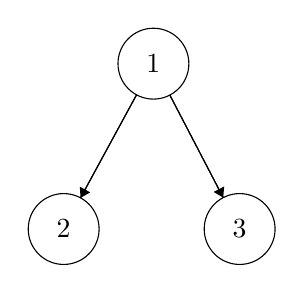
\begin{tikzpicture}[scale=0.15]
\tikzstyle{every node}+=[inner sep=0pt]
\draw [black] (38.9,-25.5) circle (3);
\draw (38.9,-25.5) node {$1$};
\draw [black] (31.3,-39.5) circle (3);
\draw (31.3,-39.5) node {$2$};
\draw [black] (46.2,-39.5) circle (3);
\draw (46.2,-39.5) node {$3$};
\draw [black] (37.47,-28.14) -- (32.73,-36.86);
\fill [black] (32.73,-36.86) -- (33.55,-36.4) -- (32.67,-35.92);
\draw [black] (32.73,-36.86) -- (37.47,-28.14);
%\fill [black] (37.47,-28.14) -- (36.65,-28.6) -- (37.53,-29.08);
\draw [black] (40.29,-28.16) -- (44.81,-36.84);
\fill [black] (44.81,-36.84) -- (44.89,-35.9) -- (44,-36.36);
\draw [black] (44.81,-36.84) -- (40.29,-28.16);
%\fill [black] (40.29,-28.16) -- (40.21,-29.1) -- (41.1,-28.64);
\end{tikzpicture}


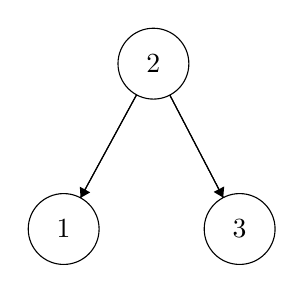
\begin{tikzpicture}[scale=0.15]
\tikzstyle{every node}+=[inner sep=0pt]
\draw [black] (38.9,-25.5) circle (3);
\draw (38.9,-25.5) node {$2$};
\draw [black] (31.3,-39.5) circle (3);
\draw (31.3,-39.5) node {$1$};
\draw [black] (46.2,-39.5) circle (3);
\draw (46.2,-39.5) node {$3$};
\draw [black] (37.47,-28.14) -- (32.73,-36.86);
\fill [black] (32.73,-36.86) -- (33.55,-36.4) -- (32.67,-35.92);
\draw [black] (32.73,-36.86) -- (37.47,-28.14);
%\fill [black] (37.47,-28.14) -- (36.65,-28.6) -- (37.53,-29.08);
\draw [black] (40.29,-28.16) -- (44.81,-36.84);
\fill [black] (44.81,-36.84) -- (44.89,-35.9) -- (44,-36.36);
\draw [black] (44.81,-36.84) -- (40.29,-28.16);
%\fill [black] (40.29,-28.16) -- (40.21,-29.1) -- (41.1,-28.64);
\end{tikzpicture}


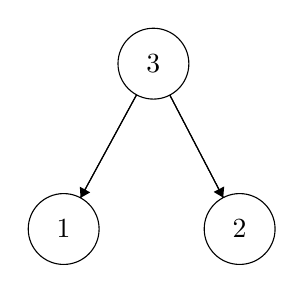
\begin{tikzpicture}[scale=0.15]
\tikzstyle{every node}+=[inner sep=0pt]
\draw [black] (38.9,-25.5) circle (3);
\draw (38.9,-25.5) node {$3$};
\draw [black] (31.3,-39.5) circle (3);
\draw (31.3,-39.5) node {$1$};
\draw [black] (46.2,-39.5) circle (3);
\draw (46.2,-39.5) node {$2$};
\draw [black] (37.47,-28.14) -- (32.73,-36.86);
\fill [black] (32.73,-36.86) -- (33.55,-36.4) -- (32.67,-35.92);
\draw [black] (32.73,-36.86) -- (37.47,-28.14);
%\fill [black] (37.47,-28.14) -- (36.65,-28.6) -- (37.53,-29.08);
\draw [black] (40.29,-28.16) -- (44.81,-36.84);
\fill [black] (44.81,-36.84) -- (44.89,-35.9) -- (44,-36.36);
\draw [black] (44.81,-36.84) -- (40.29,-28.16);
%\fill [black] (40.29,-28.16) -- (40.21,-29.1) -- (41.1,-28.64);
\end{tikzpicture}
\end{center}


This suggests the following marvelous identity, which we will shortly explore:
\begin{equation}\label{ose-eq}
\card{\symn{3}}=\card{\aut{A}}\cdot (\mbox{the number of labeled copies of }A).
\end{equation}

\subsection*{The Orbit-Stabilizer Theorem}

%\begin{definition}
Recall that for every positive integer $k$, we write $[k]$ for $\{1,\ldots,k\}$.
%\end{definition}

\begin{definition}
For every positive integer $k$, we write $\symn{k}$ for the set of bijections from $[k]$ onto $[k]$ (also called the \emph{permutation group on} or the \emph{symmetric group on} $[k]$).
\end{definition}

The names \emph{permutation group} or \emph{symmetric group} emphasize the agebraic nature of \symn{k}. Indeed, we can think of \symn{k}\ as an algebra with a binary operation $\circ$, a unary operation $^{-1}$, and a distinguished element $e$, where, for permutations $f,g\in\symn{k}$, $f\circ g$ is the permutation resulting from the composition of $f$ and $g$, that is, $f\circ g =h$ if and only if for every $i\in [k]$, $h(i) = f(g(i))$; $f^{-1}$ is the permutation which is the inverse of $f$; and $e$ stands for the identity function on $[k]$. With these understandings, you can verify that \symn{k}\ is a group\footnote{These conditions (associativity, identity, inverse, closure) are the axioms for a \emph{group}, which is a fundamental and widely applicable concept in algebra. Group Theory, the part of mathematics which studies groups, is a hugely influential and interesting field. MATH 370 is Penn's introductory group theory course. }: 

\begin{itemize}
\item   
$\circ$ is an associative operation, that is, $(f\circ g)\circ h= f\circ (g\circ h)$, for all $f,g\in\symn{k}$;
\item
 $e$ is an identity with respect to $\circ$, that is, $e\circ f = f\circ e = f$, for all $f\in\symn{k}$; and 
 \item
 $f\circ f^{-1} = f^{-1}\circ f = e$, for all $f\in\symn{k}$.
 \item Permutations are closed under $\circ$, that is, $f \circ g$ is a permutation for all $f, g \in \symn{k}$. 
\end{itemize} 

\begin{aside}
Prove that each of these conditions holds. 
\end{aside}

\begin{definition}
We write $\sgraphn{k}$ ($=\modn{\sg}{k}$) for the set of simple graphs $A$ with $U^A = [k]$.
\end{definition}
\iffalse
\begin{definition}
For each $f\in\symn{k}$ and $A\in\sgraphn{k}$, we define $f[A]$ (called the \emph{image of the graph $A$ under $f$}) to be the graph with universe $[k]$ and edge-set
\[
    L^{f[A]} := \{\op{f(i)}{f(j)} \mid \op{i}{j} \in L^A\}
\]
Note that $f$ is an isomorphism of $A$ onto $f[A]$.
\end{definition}
\fi
Recall that for each $f\in\symn{k}$ and $A\in\sgraphn{k}$, $f[A]$ is the image of the graph $A$ under $f$.
This is an example of a \emph{group action} - the group \symn{k} \emph{acts on} the set \sgraphn{k}\ via the assignment of $f[A]$ to $A$. 

\begin{aside}
    Just as with groups, group actions are axiomatized by a few simple conditions. To verify that this is indeed a group action, show that for all $A\in\sgraphn{k}$ and $f,g\in\symn{k}$ the following properties hold:
    \begin{itemize}
    \item
    $(f\circ g)[A]=f[g[A]]$, and 
    \item
    $e[A]=A$.
    \end{itemize}    
\end{aside}


Recall that \aut{A}\ is the set of automorphisms of $A$. In the current context, for $A\in \sgraphn{k}$, \aut{A}\ is often called the \emph{stabilizer} of $A$, since $f\in\aut{A}$ if and only if $f[A] =A$. 

\begin{definition}
The \emph{orbit of} $A$  under the action of \symn{k}\ (written $\orb{A}{\symn{k}}$) is $\{h[A]\mid h\in\symn{k}\}$. 

In other words, the orbit of $A$ under \symn{k} is the set of $B\in\sgraphn{k}$ such  that $A\cong B$. \end{definition}

The following result is a special case of the \emph{Orbit-Stabilizer Theorem}.
\begin{theorem}\label{orb-stab-thm}
For all $A\in\sgraphn{k}$,
\[
\card{\symn{k}}=\card{\orb{A}{\symn{k}}}\cdot\card{\aut{A}}.
\]
\end{theorem}

\emph{Proof}:
Let $A\in\sgraphn{k}$. We define an equivalence relation $\sim$ on $\symn{k}$: for all $f,g\in\symn{k}$, $f\sim g$ if and only if $(f^{-1}\circ g)\in\aut{A}$. 

\begin{aside}
    Verify that $\sim$ is an equivalence relation, for example, it is reflexive (that is, $f\sim f$), because $f^{-1}\circ f = e$ and $e\in \aut{A}$. Continue and show $\sim$ is symmetric and transitive.
\end{aside}

%To establish the theorem, we prove two lemmata. 

We establish the following two claims about $\sim$ from which the Theorem follows immediately.
\begin{enumerate}
\item
each equivalence class of $\sim$ has size $\card{\aut{A}}$, and
\item
the number of equivalence classes of $\sim$ is $\card{\orb{A}{\symn{k}}}$.
\end{enumerate}
\emph{Ad} claim 1: Fix $f\in\symn{k}$. For each $h\in\aut{A}$ there is a unique $g\in\symn{k}$ such that $f^{-1}\circ g = h$. It follows at once that there is a bijection between $\{g\mid f\sim g\}$ and \aut{A}.

\begin{aside}
    Use the group axioms to first prove that inverses in a group are unique (that is, for any $f$ in a group, there is a unique element $f^{-1}$ such that $f \circ f^{-1} = e = f^{-1} \circ f$, where $e$ is the identity element).

    Using that fact, verify that for each fixed $f, h \in \symn{k}$, there is a unique $g \in \symn{k}$ such that $f^{-1}\circ g = h$. 
\end{aside}

\emph{Ad} claim 2: We show that for every $f,g\in\symn{k}$ $f[A]=g[A]$ if and only if $f\sim g$. We prove each direction of the bi-conditional. 

First, suppose suppose $f\sim g$. Then 
$f^{-1}\circ g \in \aut{A}$. It follows that $(f^{-1}\circ g)[A] = A$ and hence that $f[(f^{-1}\circ g)[A]] = f[A]$. So $(f\circ(f^{-1}\circ g))[A] = f[A]$, and then by associativity $((f\circ f^{-1})\circ g)[A] = f[A]$. As $f \circ f^{-1} = e$, we have $(e\circ g)[A] = f[A]$ from which it follows that $g[A]=f[A]$. 

In the other direction, suppose $f[A]=g[A]$. Then, $f^{-1}[f[A]]=f^{-1}[g[A]]$. Hence, $(f^{-1}\circ f)[A]=(f^{-1}\circ g)[A]$. Hence, $(f^{-1}\circ g)[A]=e[A]= A$. Hence, $f^{-1}\circ g\in \aut{A}$, that is, $f\sim g$. Thus, there is a bijection between the equivalence classes of $\sim$ and $\orb{A}{\symn{k}}$. \qed

We now have the explanation of identity (\ref{ose-eq}), since 
\[
\card{\orb{A}{\symn{k}}}=\mbox{the number of labeled copies of }A.
\]

We illustrate the use of Theorem \ref{orb-stab-thm} via an application to counting structures that satisfy a given schema. %In order to test out our new theorem, %\footnote{Look mom, I got a new Theorem for my birthday! I wanna play with it immediately!} let's use it for some counting. 
Let $S$ be the conjunction of $\sg$ and $\oner$, that is, a graph $A$ satisfies $S$ if and only if $A$ is a 1-regular, simple graph. As we discussed earlier, every such finite graph $A$ has an even number, say $2n$, of nodes; moreover, if $A,B\models S$ and $\card{U^A}=\card{U^B}$, then $A$ is isomorphic to $B$. We will calculate the value of $\modn{S}{2n}$ in two ways - one way using the Orbit-Stabilizer Theorem, and the other directly. 

\subsubsection*{Via the Orbit-Stabilizer Theorem}
Let $A\in\modn{S}{2n}$. As we've just noted above, if $B\in\modn{S}{2n}$, then $A\cong B$. It follows at once that 
\begin{equation}\label{vos-eq}
\modn{S}{2n}=\orb{A}{\symn{2n}}.
\end{equation}
Let's calculate $\card{\aut{A}}$, since Theorem \ref{orb-stab-thm} will then allow us to calculate $\card{\modn{S}{2n}}$. Observe that $A$ consists of $n$ independent edges. Imagine them standing upright and lined up horizontally in some order. 

\begin{center}
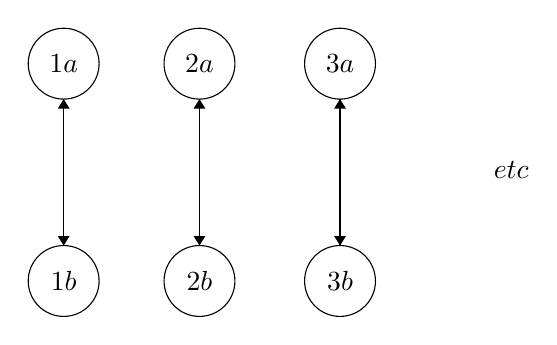
\begin{tikzpicture}[scale=0.15]
\tikzstyle{every node}+=[inner sep=0pt]
\draw [black] (22.2,-16) circle (3);
\draw (22.2,-16) node {$1a$};
\draw [black] (22.2,-34.4) circle (3);
\draw (22.2,-34.4) node {$1b$};
\draw [black] (33.7,-16) circle (3);
\draw (33.7,-16) node {$2a$};
\draw [black] (33.7,-34.4) circle (3);
\draw (33.7,-34.4) node {$2b$};
\draw [black] (45.6,-16) circle (3);
\draw (45.6,-16) node {$3a$};
\draw [black] (45.6,-34.4) circle (3);
\draw (45.6,-34.4) node {$3b$};
\draw (60.1,-25) node {$etc$};
\draw [black] (22.2,-19) -- (22.2,-31.4);
\fill [black] (22.2,-31.4) -- (22.7,-30.6) -- (21.7,-30.6);
\draw [black] (22.2,-31.4) -- (22.2,-19);
\fill [black] (22.2,-19) -- (21.7,-19.8) -- (22.7,-19.8);
\draw [black] (33.7,-19) -- (33.7,-31.4);
\fill [black] (33.7,-31.4) -- (34.2,-30.6) -- (33.2,-30.6);
\draw [black] (33.7,-31.4) -- (33.7,-19);
\fill [black] (33.7,-19) -- (33.2,-19.8) -- (34.2,-19.8);
\draw [black] (45.6,-19) -- (45.6,-31.4);
\fill [black] (45.6,-31.4) -- (46.1,-30.6) -- (45.1,-30.6);
\draw [black] (45.6,-31.4) -- (45.6,-19);
\fill [black] (45.6,-19) -- (45.1,-19.8) -- (46.1,-19.8);
\end{tikzpicture}
\end{center}

Now any permutation of the edges generates an automorphism of $A$. Moreover, in the process of permuting the edges, we have for each edge a choice whether to ``flip'' the edge or not. Since there are $n!$ permutations of the $n$ edges, and $2^n$ choices of which set of edges to flip, there are a total of $n!\cdot 2^n$ automorphisms of $A$. Hence, by Theorem \ref{orb-stab-thm} and equation (\ref{vos-eq}), 
 \[
 \card{\modn{S}{2n}}= (2n)!/n!\cdot 2^n.
 \]

\subsubsection*{Directly}
Here is a second direct method of calculating $\card{\modn{S}{2n}}$ which, thankfully, yields the same result.%\footnote{If it didn't, we'd have to agree that our new toy was broken, and would probably have a miserable rest of the day what with the inconvenience of having to return it and all.}. 
We construct a member $A$ of $\modn{S}{2n}$ as follows. We successively choose the $n$ independent edges that constitute $A$. So for the first edge, we have $\binom{2n}{2}$ choices of a pair of nodes between which to place an edge, and for the second edge, we have $\binom{2n-2}{2}$ choices, .... So the number of ways we can choose a sequence of $n$ independent edges is
\[
\binom{2n}{2}\cdot\binom{2n-2}{2}\cdots\binom{4}{2}\cdot\binom{2}{2}= \frac{(2n)!}{2^n}.
\]
Now any \emph{set} of $n$ edges chosen via this process will appear as the result of $n!$ such sequences of choices; thus, the total number of members of $\modn{S}{2n}$ we can construct is 
\[
\frac{(2n)!}{n!\cdot 2^n}.
\]
\newpage

\subsection{Definability}
Up to this point we have neglected schemata containing free variables. We will now correct this oversight. 

Consider the structure $A$ (which should look familiar) defined by
\[
    U^A = [3], L^A=\{\op{1}{2},\op{1}{3}\}
\]
Define the schema
\[
    S(x):\ \ \ \neg(\exists y)Lyx.
\]
$S(x)$ picks out $1$ uniquely from the structure $A$, because $1$ is the only element in $U^A$ which does not have an incoming edge. Symbolically, we express this as
\[
\{a\in U^A\mid A\models S[x|a]\}=\{1\}.
\]

$S(x)$ expresses the property of having in-degree zero. Since we only consider properties extensionally, we can also say that, in a given structure, $S(x)$ defines the set of nodes of in-degree zero. The concept of definability is central in logic (and many other disciplines). We enshrine it in a definition.

\begin{definition}
Let $S(x)$ be a schema with one free variable $x$ and let $A$ be a structure.
We define $S[A]=\{a\in U^A\mid A\models S[x|a]\}$. In other words, $S[A]$ is the set of nodes $a \in A$ that satisfy the schema $S(x)$ in $A$ when we assign $a$ to the variable $x$. We call $S[A]$ the \emph{set defined by} $S(x)$ in $A$.
\end{definition}

\begin{definition}
We say a set $V\subseteq U^A$ is a \emph{definable subset of} $A$ if and only if there is a schema $S(x)$ such that $S[A]=V$.
\end{definition}

Note that the set $\{2,3\}$ is defined by the schema
\[
S'(x):\ \ \ \neg(\exists y)Lxy.
\]

Are either of the sets $\{2\}$ or $\{3\}$ definable as subsets of $A$? Try as you might, you won't find a schema which picks out either $2$ or $3$ individually. Intuitively, this is because the nodes labelled 2 and 3 appear to be ``indistinguishable from a structural point of view''. Backing up this notion of indistinguishability, we see that the function $h$ mapping 1 to 1, 2 to 3, and 3 to 2, is an automorphism of $A$ which happens to exchange $2$ and $3$. The relevance of this to the question of definability is the content of the following fundamental theorem.

\subsubsection*{The Automorphism Theorem, Orbits, and Definability over finite structures}
\begin{theorem}\label{aut-thm}
Let $A$ be a graph and $h\in\aut{A}$. For every $a\in U^A$ and every schema $S(x)$,
\[
A\models S[x|a]\mbox{ if and only if }A\models S[x|h(a)]. 
\]
\end{theorem}

Theorem \ref{aut-thm} enables us to give a characterization of the definable subsets of finite structures. 
If $f$ is a function with domain $U$ and $V\subseteq U$, we define $f[V]=\{f(a)\mid a\in V\}$ (the $f$ \emph{image} of $V$). With this notation in hand, we can now state a corollary to Theorem \ref{aut-thm} which bears on definability.
\begin{corollary}\label{aut-def-cor}
Let $A$ be a graph and $h\in\aut{A}$. If $V$ is a definable subset of $A$, then $h[V]=V$.
\end{corollary}
Thus, in order to show that $V$ is \emph{not} a definable subset of $A$ it suffices to exhibit an $h\in\aut{A}$ and $a\in V$ such that $h(a)\not\in V$. Moreover, in the case of finite structures, the converse of Corollary \ref{aut-def-cor} is true.
\begin{theorem}\label{fin-aut-def-thm}
Let $A$ be a finite graph and $V\subseteq U^A$. $V$ is a definable subset of $A$, if for every $h\in\aut{A}$, $h[V]=V$.
\end{theorem}

\subsection*{Orbits and Definability over finite structures}
In order to prove Theorem \ref{fin-aut-def-thm}, and to apply it to questions of counting definable sets, the following definitions will be useful. 

\begin{definition}
The \emph{orbit of a node} $a\in U^A$ \emph{under the action of} $\aut{A}$ is the set of all possible images of $a$ under actions $f \in \aut{A}$. Symbolically,
\[
\orb{a}{\aut{A}}=\{h(a)\mid h\in\aut{A}\}.
\]
\end{definition}

\begin{definition}
The \emph{orbits of $A$} is the set of all orbits of individual elements $a \in A$. Symbolically:
\[
    \autorbs{A}=\{\orb{a}{\aut{A}}\mid a\in U^A\}
\]
\end{definition}

As a corollary to Corollary \ref{aut-def-cor} and Theorem \ref{fin-aut-def-thm} we have:
\begin{corollary}\label{def-orbs-cor}
Let $A$ be a finite graph and $V\subseteq U^A$. $V$ is a definable subset of $A$ if and only if either $V=\emptyset$ or there is a sequence of sets $O_1, \ldots,O_k$, where each $O_i\in\autorbs{A}$, and $V = O_1\cup\ldots\cup O_k$.
\end{corollary}

\begin{aside}
    Use Corollary \ref{aut-def-cor} and Theorem \ref{fin-aut-def-thm} to prove this. 
\end{aside}

It follows at once from Corollary \ref{def-orbs-cor}, that if $A$ is a finite graph, then the number of definable subsets of $A$ is $2^{\card{\autorbs{A}}}$. 



\subsubsection*{An example: definable subsets of simple graphs with four nodes}

To make this all a little bit more concrete, lets give a complete analysis of the definable subsets of simple graphs with four nodes.

Let's classify all members of $\modn{\sg}{4}$ up to isomorphism - that is, exhibit examples of all the size-4 simple graphs. There is a single such graph with no edges which we will call $A_1$. This looks like

\[
    \begin{array}{|l|}
    \hline
    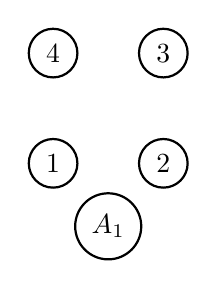
\begin{tikzpicture}
[scale=.2]
\begin{scope}[every node/.style={circle,thick,draw}]
    \node (1) at (0,4) {1};
    \node (2) at (7,4) {2};
    \node (3) at (7,11) {3};
    \node (4) at (0,11) {4};
   \node(A) at (3.5,0) {$A_1$};
\end{scope}
\end{tikzpicture}\\
\hline
\end{array}
\]

By symmetry, there is also a single maximal size-4 graph with 6 edges

\[
    \begin{array}{|l|}
    \hline
    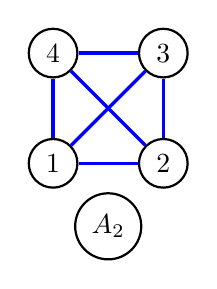
\begin{tikzpicture}
[scale=.2]
\begin{scope}[every node/.style={circle,thick,draw}]
    \node (1) at (0,4) {1};
    \node (2) at (7,4) {2};
    \node (3) at (7,11) {3};
    \node (4) at (0,11) {4};
   \node(A) at (3.5,0) {$A_2$};
\end{scope}

\begin{scope}[%>={Stealth[black]},
              every node/.style={fill=white,circle},
              every edge/.style={draw=blue,very thick}]
     \draw (1) edge  (2);
     \draw (2) edge  (3);
     \draw (3) edge  (4);
     \draw (4) edge  (1);
     \draw (4) edge  (2);
     \draw (3) edge  (1);
             
\end{scope}
\end{tikzpicture}\\
\hline
\end{array}
\]

Up to isomorphism, there is one size-4 graph with a single edge (since we only care about equivalence up to isomorphism, the labels of the ends of the single edge don't matter). By symmetry, there is a single size-4 graph with 5 edges. 

\[
    \begin{array}{|l|l|}
        \hline
        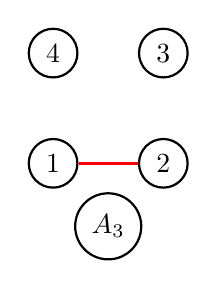
\begin{tikzpicture}
        [scale=.2]
        \begin{scope}[every node/.style={circle,thick,draw}]
            \node (1) at (0,4) {1};
            \node (2) at (7,4) {2};
            \node (3) at (7,11) {3};
            \node (4) at (0,11) {4};
           \node(A) at (3.5,0) {$A_3$};
        \end{scope}

        \begin{scope}[%>={Stealth[black]},
                      every node/.style={fill=white,circle},
                      every edge/.style={draw=red,very thick}]
              \draw (1) edge  (2);
             %\draw (2) edge  (3);
             %\draw (3) edge  (4);
             %\draw (4) edge  (1);
             %\draw (4) edge  (2);
             %\draw (3) edge  (1);             
        \end{scope}
        \end{tikzpicture}
        &
        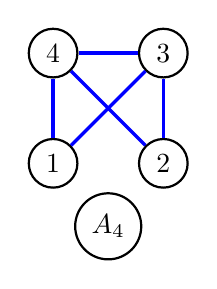
\begin{tikzpicture}
        [scale=.2]
        \begin{scope}[every node/.style={circle,thick,draw}]
            \node (1) at (0,4) {1};
            \node (2) at (7,4) {2};
            \node (3) at (7,11) {3};
            \node (4) at (0,11) {4};
           \node(A) at (3.5,0) {$A_4$};
        \end{scope}

        \begin{scope}[%>={Stealth[black]},
                      every node/.style={fill=white,circle},
                      every edge/.style={draw=blue,very thick}]
             %\draw (1) edge  (2);
             \draw (2) edge  (3);
             \draw (3) edge  (4);
             \draw (4) edge  (1);
             \draw (4) edge  (2);
             \draw (3) edge  (1);
                     
        \end{scope}
        \end{tikzpicture}\\
        \hline
    \end{array}
\]

There are two non-isomorphic size-4 graphs with two edges, and similarly two such graphs with 4 edges. 

\[
    \begin{array}{|l|l|}
    \hline

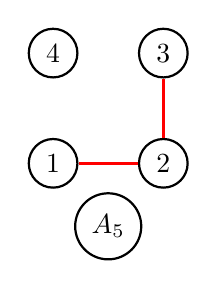
\begin{tikzpicture}
[scale=.2]
\begin{scope}[every node/.style={circle,thick,draw}]
    \node (1) at (0,4) {1};
    \node (2) at (7,4) {2};
    \node (3) at (7,11) {3};
    \node (4) at (0,11) {4};
   \node(A) at (3.5,0) {$A_5$};
\end{scope}

\begin{scope}[%>={Stealth[black]},
              every node/.style={fill=white,circle},
              every edge/.style={draw=red,very thick}]
\draw (1) edge  (2);
     \draw (2) edge  (3);
     %\draw (3) edge  (4);
     %\draw (4) edge  (1);
     %\draw (4) edge  (2);
     %\draw (3) edge  (1);             
\end{scope}
\end{tikzpicture}
&
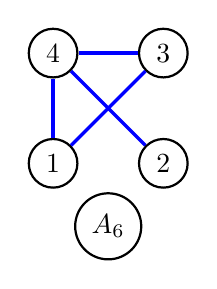
\begin{tikzpicture}
[scale=.2]
\begin{scope}[every node/.style={circle,thick,draw}]
    \node (1) at (0,4) {1};
    \node (2) at (7,4) {2};
    \node (3) at (7,11) {3};
    \node (4) at (0,11) {4};
   \node(A) at (3.5,0) {$A_6$};
\end{scope}

\begin{scope}[%>={Stealth[black]},
              every node/.style={fill=white,circle},
              every edge/.style={draw=blue,very thick}]
%\draw (1) edge  (2);
%     \draw (2) edge  (3);
     \draw (3) edge  (4);
     \draw (4) edge  (1);
     \draw (4) edge  (2);
     \draw (3) edge  (1);
             
\end{scope}
\end{tikzpicture}
\\
\hline
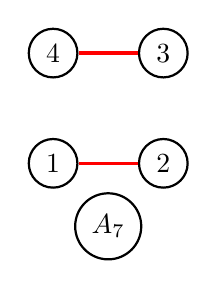
\begin{tikzpicture}
[scale=.2]
\begin{scope}[every node/.style={circle,thick,draw}]
    \node (1) at (0,4) {1};
    \node (2) at (7,4) {2};
    \node (3) at (7,11) {3};
    \node (4) at (0,11) {4};
   \node(A) at (3.5,0) {$A_7$};
\end{scope}

\begin{scope}[%>={Stealth[black]},
              every node/.style={fill=white,circle},
              every edge/.style={draw=red,very thick}]
\draw (1) edge  (2);
     %\draw (2) edge  (3);
     \draw (3) edge  (4);
     %\draw (4) edge  (1);
     %\draw (4) edge  (2);
     %\draw (3) edge  (1);             
\end{scope}
\end{tikzpicture}
&
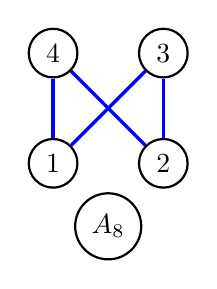
\begin{tikzpicture}
[scale=.2]
\begin{scope}[every node/.style={circle,thick,draw}]
    \node (1) at (0,4) {1};
    \node (2) at (7,4) {2};
    \node (3) at (7,11) {3};
    \node (4) at (0,11) {4};
   \node(A) at (3.5,0) {$A_8$};
\end{scope}

\begin{scope}[%>={Stealth[black]},
              every node/.style={fill=white,circle},
              every edge/.style={draw=blue,very thick}]
%\draw (1) edge  (2);
     \draw (2) edge  (3);
%     \draw (3) edge  (4);
     \draw (4) edge  (1);
     \draw (4) edge  (2);
     \draw (3) edge  (1);
     \end{scope}
\end{tikzpicture}

    \\
    \hline
    \end{array}
\]

Lastly, there are three non-isomorphic size-4 simple graphs with three edges. $A_9$ and $A_{10}$ are complements of each other, whereas $A_{11}$, is its own complement. 

\[
    \begin{array}{|l|l|l|}
    \hline
    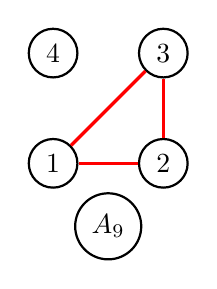
\begin{tikzpicture}
[scale=.2]
\begin{scope}[every node/.style={circle,thick,draw}]
    \node (1) at (0,4) {1};
    \node (2) at (7,4) {2};
    \node (3) at (7,11) {3};
    \node (4) at (0,11) {4};
   \node(A) at (3.5,0) {$A_9$};
\end{scope}

\begin{scope}[%>={Stealth[black]},
              every node/.style={fill=white,circle},
              every edge/.style={draw=red,very thick}]
\draw (1) edge  (2);
     \draw (2) edge  (3);
%     \draw (3) edge  (4);
%     \draw (4) edge  (1);
%     \draw (4) edge  (2);
     \draw (3) edge  (1);
     \end{scope}
\end{tikzpicture}
&
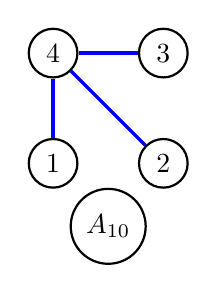
\begin{tikzpicture}
[scale=.2]
\begin{scope}[every node/.style={circle,thick,draw}]
    \node (1) at (0,4) {1};
    \node (2) at (7,4) {2};
    \node (3) at (7,11) {3};
    \node (4) at (0,11) {4};
   \node(A) at (3.5,0) {$A_{10}$};
\end{scope}

\begin{scope}[%>={Stealth[black]},
              every node/.style={fill=white,circle},
              every edge/.style={draw=blue,very thick}]
%\draw (1) edge  (2);
%     \draw (2) edge  (3);
     \draw (3) edge  (4);
     \draw (4) edge  (1);
     \draw (4) edge  (2);
%     \draw (3) edge  (1);
             
\end{scope}
\end{tikzpicture}
&
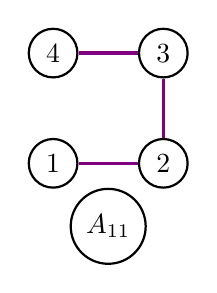
\begin{tikzpicture}
[scale=.2]
\begin{scope}[every node/.style={circle,thick,draw}]
    \node (1) at (0,4) {1};
    \node (2) at (7,4) {2};
    \node (3) at (7,11) {3};
    \node (4) at (0,11) {4};
   \node(A) at (3.5,0) {$A_{11}$};
\end{scope}

\begin{scope}[%>={Stealth[black]},
              every node/.style={fill=white,circle},
              every edge/.style={draw=violet,very thick}]
 \draw (1) edge  (2);
     \draw (2) edge  (3);
     \draw (3) edge  (4);
%     \draw (4) edge  (1);
 %    \draw (4) edge  (2);
  %   \draw (3) edge  (1);
     \end{scope}
\end{tikzpicture}
\\
\hline

\end{array}
\]

\begin{aside}
    Verify that these are all of the non-isomorphic graphs of size 4 by beginning with 4 empty nodes and iteratively constructing all non-isomorphic graphs with increasing number of edges. 
\end{aside}

Now that we have a maximal collection of pairwise non-isomorphic graphs in $\modn{\sg}{4}$, we can calculate $\card{\orb{A_i}{\symn{4}}}$ and $\card{\aut{A_i}}$ for each $1\leq i\leq 11$. 

\begin{aside}
    Prove that $\aut{A} = \aut{A^c}$ for every simple graph $A$. 

    From this, it follows that if $A_i$ and $A_j$ are complements, we have that $\card{\aut{A_i}} = \card{\aut{A_j}}$ and moreover $\card{\orb{A_i}{\symn{4}}} = \card{\orb{A_j}{\symn{4}}}$. This will make our counting easier, because it nearly halves the amount of work we have to do. 
\end{aside}

What is $\card{\orb{A_1}{\symn{4}}}$, or in other words, how many distinct ways can we place 0 edges onto 4 labelled nodes? There is only one way to do this, so $\card{\orb{A_1}{\symn{4}}} = 1$. What is $\card{\aut{A_1}}$, or in other words, how many ways can we permute the edges of $A_1$ once the edges are fixed in place? There are no edges, so any permutation of the nodes (of which there are $4! = 24$) is valid. It follows that $\card{\aut{A_1}} = 24$. By symmetry, it follows that $\card{\orb{A_2}{\symn{4}}} = 1$ and $\card{\aut{A_2}} = 24$ as well. 

As another example, let's calculate $\card{\orb{A_5}{\symn{4}}}$ and $\card{\aut{A_5}}$ (and hence the values for $A_6$ as well). There are $4 \cdot 3 = 12$ ways of placing 2 edges onto 4 nodes such that the two edges are connected as in $A_5$, as there are $4$ choices for the ``central'' node and $\binom{3}{2} = 3$ choices for which two other nodes (which we will call \emph{leaves}) get connected to the central node. It follows that $\card{\orb{A_5}{\symn{4}}} = \card{\orb{A_6}{\symn{4}}} = 12$. Once the edges have been fixed, there are two possible automorphisms: the identity automorphism, and automorphism which exchanges the two leaf nodes. It follows that $\card{\aut{A_5}} = \card{\aut{A_6}} = 2$. 

Without too much extra work, we arrive at the complete table:

\[
\begin{array}{|c|c|c|}
\hline
A_i  & \card{\orb{A_i}{\symn{4}}} & \card{\aut{A_i}}\\
\hline
A_1 & 1 & 24\\
\hline
A_2 & 1 & 24 \\
\hline
A_3 & 6 & 4\\
\hline
A_4 & 6 & 4\\
\hline
A_5 & 12 & 2\\
\hline
A_6 & 12 & 2\\
\hline
A_7 & 3 & 8 \\
\hline
A_8 & 3 & 8 \\
\hline
A_9 & 4 & 6 \\
\hline
A_{10} & 4 & 6 \\
\hline
A_{11} & 12 & 2\\
\hline
\end{array}
\]

\begin{aside}
    Calculate each of the values not discussed in the examples. 
\end{aside}

Note the ``verification'' of the result predicted by the Orbit-Stabilizer Theorem: $\card{\orb{A_i}{\symn{4}}} \cdot \card{\aut{A_i}} = \card{\symn{4}} (= 24)$.
%\subsection{Addendum}

By Corollary \ref{def-orbs-cor}, calculating $\autorbs{A_i}$ suffices to determine which sets are definable in each $A_i$. 

\begin{example}
What is $\autorbs{A_5}$?
\end{example}
To determine $\autorbs{A_5}$, it suffices to determine the orbits of individual elements. The orbit of node $4$ is $\{4\}$, as it is the only isolated node. The orbit of $2$ is $\{2\}$, as it is the only node of degree two. The orbit of $1$ is $\{1, 3\}$ as $1$ is a leaf node, and we had an automorphism that exchanged leaf nodes. As the set of orbits partition the nodes, the orbit of $3$ is $\{1, 3\}$ as well. It follows that $\autorbs{A_5} = \{\{2\}, \{4\}, \{1, 3\}\}$. 

\begin{aside}
A \emph{partition} of a set $S$ is a collection $\mathcal{P}$ of subsets of $S$ such that: (1) every $s \in S$ is in some $P \in \mathcal{P}$, and (2) if $P, P' \in \mathcal{P}$ and $P \cap P' \neq 0$, then $P = P'$ (ie, no distinct elements of $\mathcal{P}$ overlap).

$\autorbs{A}$ trivially satisfies condition (1), since every node in $A$ is in its own orbit. Complete the proof $\autorbs{A}$ is a partition of the nodes of $A$ by showing that condition (2) holds. 
\end{aside}  

With a little more work, we arrive at the following table. 
\[
\begin{array}{l l}
A_i & \autorbs{A_i}\\
\hline
A_1, A_2 & \{[4]\}\\
A_3, A_4 & \{\{1,2\},\{3,4\}\}\\
A_5, A_6 & \{\{2\},\{4\},\{1,3\}\}\\
A_7, A_8 & \{[4]\}\\
A_9, A_{10} & \{\{1,2,3\},\{4\}\}\\
A_{11} & \{\{1,4\},\{2,3\}\}
\end{array}
\]

\begin{aside}
    Derive each of the above sets of orbits yourself, to make sure all the concepts fit into place. 
\end{aside}

\subsection*{Proofs for Theorem \ref{aut-thm} and Theorem \ref{fin-aut-def-thm}}
We now develop the necessary technology in order to give proof sketches for Theorem \ref{aut-thm} and Theorem \ref{fin-aut-def-thm}.  

\subsubsection*{Automorphisms and Degree}
Let $A$ be a graph and $a\in U^A$. Recall that the \emph{neighborhood of} $a$ in $A$ is $\nbh{a}{A} := \{b\in U^A\mid\op{a}{b}\in L^A\}$. The \emph{degree of} $a$ in $A$ is $\dg{a}{A} := \card{\{b\in U^A\mid\op{a}{b}\in L^A\}}$. We have the following fact:
\begin{proposition}
For every graph $A$, $a\in U^A$, and $h\in\aut{A}$,
\[
h[\nbh{a}{A}]=\nbh{h(a)}{A}.
\]
Hence,
\[
\dg{a}{A} = \dg{h(a)}{A}. 
\]
In other words, automorphisms preserve degree. 
\end{proposition}

\begin{aside}
    Show that this follows from the definition of an automorphism.
\end{aside}

\begin{definition}
    We say that a graph $A$ is \emph{rigid} if and only if $\aut{A}=\{e\}$, that is, $A$ has no non-trivial automorphisms.
\end{definition}

It follows at once from Theorem \ref{fin-aut-def-thm} that if $A$ is a finite rigid structure and $V\subseteq U^A$, then $V\in\Def{A}$.

\begin{aside}
    Why? Think about what $\aut{A}=\{e\}$ implies about the orbit of each element (and hence $\autorbs{A}$). 
\end{aside}

\begin{aside}
    No member of $\modn{\sg}{4}$ is rigid, as each has non-trivial automorphisms. This suggests an interesting question: ``what is the least $n$ such that $\modn{\sg}{n}$ contains a rigid graph?''
\end{aside}

\subsubsection*{Proof Sketch of Theorem \ref{fin-aut-def-thm}}
We aim to show that for every finite graph $A$, $V \subset A$ is definable iff every automorphism $h \in \aut{A}$ leaves $V$ unchanged. The generalization to structures interpreting multiple polyadic predicates is straightforward.

First, suppose $A$ is a finite graph, $a\in U^A$, and $V=\orb{A}{\aut{A}}$. We construct a schema $S(x)$ such that $S[A]=V$ by . We may suppose without loss of generality that $U^A=[k]$ for some $k\in\mathbb{Z}^+$ and that $a=1$. For each $1\leq i,j\leq k$, let the schema $S_{i,j}$ be $Lx_ix_j$ if $\op{i}{j}\in L^A$, and $\neg Lx_ix_j$ otherwise. Let $S(x)$ be the schema
\[
(\exists x_2)\ldots(\exists x_k)(\bigwedge_{1\leq i,j\leq k}S_{i,j}\wedge\bigwedge_{1\leq i<j\leq k}x_i\neq x_j\wedge(\forall y)\bigvee_{1\leq i\leq k} y=x_i).
\] 
Let $a_1,\dots,a_k$ be a sequence of nodes from $U^A$ and observe that
\[
A\models(\bigwedge_{1\leq i,j\leq k}S_{i,j}\wedge\bigwedge_{1\leq i<j\leq k}x_i\neq x_j\wedge(\forall y)\bigvee_{1\leq i\leq k} y=x_i)[(x_1|a_1),\ldots,(x_k|a_k)]
\]
if and only if the function mapping $i$ to $a_i$ is an automorphism of $A$. \qed


Theorem \ref{aut-thm} is a corollary of the following more general result concerning isomorphisms of structures.
\begin{theorem}\label{iso-thm}
Suppose $A$ and $B$ are structures and $f$ is an isomorphism of $A$ onto $B$. Then for every schema $S(x_1,\ldots,x_k)$ and sequence of elements $a_1,\dots,a_k\in U^A$,
\begin{equation}\label{iso-eq}
A\models S[(x_1|a_1),\ldots,(x_k|a_k)]\mbox{ iff }B\models S[(x_1|f(a_1)),\ldots,(x_k|f(a_k))].
\end{equation}
\end{theorem}

{\bf Proof sketch of Theorem \ref{iso-thm}}:
We give the argument for graphs; the generalization to structures interpreting multiple polyadic predicates is straightforward.
The argument proceeds by induction on the syntactic structure of schemata. The base case verifies (\ref{iso-eq}) for atomic schemata, that is, schemata of the form $Lx_ix_j$ or $x_i=x_j$, for some $i,j$. In this case, the verification follows directly from the hypothesis that $f$ is an isomorphism from $A$ onto $B$, in particular, that it is edge-preserving and injective.

Suppose $S$ is a truth-functional combination, for example the conjunction, of schemata $S'$ and $S''$, where, as hypothesis of induction, (\ref{iso-eq}) holds for both $S'$ and $S''$. Then,
\[
\begin{array}{lc}
A\models S[(x_1|a_1),\ldots,(x_k|a_k)] & \mbox{ iff}\\
A\models S'[(x_1|a_1),\ldots,(x_k|a_k)]\mbox{ and }A\models S''[(x_1|a_1),\ldots,(x_k|a_k)] & \mbox{ iff}\\
B\models S'[(x_1|f(a_1)),\ldots,(x_k|f(a_k))]\mbox{ and }B\models S''[(x_1|f(a_1)),\ldots,(x_k|f(a_k))] & \mbox{ iff}\\
B\models S[(x_1|f(a_1)),\ldots,(x_k|f(a_k))].
\end{array}
\]
The first and third biconditionals follow from the truth-functional semantics of conjunction, while the second follows from the induction hypothesis.

Finally, suppose that $S$ is $(\exists y)S'(x_1,\ldots,x_k,y)$ and (\ref{iso-eq}) holds for $S'$ (the universal quantifier is handled similarly). Then,
\[
\begin{array}{lc}
A\models S[(x_1|a_1),\ldots,(x_k|a_k)] & \mbox{ iff}\\
\mbox{for some $a\in U^A$ }
A\models S'[(x_1|a_1),\ldots,(x_k|a_k),(y|a)] & \mbox{ iff}\\
\mbox{for some $a\in U^A$ }
B\models S'[(x_1|f(a_1)),\ldots,(x_k|f(a_k)),(y|f(a))] & \mbox{ iff}\\
\mbox{for some $b\in U^B$ }
B\models S'[(x_1|f(a_1)),\ldots,(x_k|f(a_k)),(y|b)] & \mbox{ iff}\\
B\models S[(x_1|f(a_1)),\ldots,(x_k|f(a_k))].
\end{array}
\]
The first and fourth biconditionals follow from the semantics for the existential quantifier, the second from the induction hypothesis, and the third from the hypothesis that $f$ is an isomorphism from $A$ onto $B$, in particular, that it is
surjective. \qed 

\begin{aside}
    In the proof above, the only truth-functional connective we considered was conjunction. The other cases are handled similarly. Complete those cases yourself, either by writing out the whole argument, or by showing that a conditional can be defined in terms of some conditionals whose cases you already worked out (for example, each of the connectives can be defined in terms of $\lnot$ and $\land$, so those two cases suffice). 
\end{aside}

\begin{aside}
    Show that Theorem \ref{aut-thm} is a corollary to Theorem \ref{iso-thm}
\end{aside}

\subsection*{Definability in Infinite Structures}
We now turn away from the safe confines of the finite and present two examples pertaining to definability in infinite structures.

\subsubsection*{A Structure With Many Automorphisms: The Integers with Absolute Value}
Let $A$ be an infinite graph defined by
\[
    U^A = \mathbb{Z}, L^A = \{\op{i}{j}\mid j \mbox{ is the absolute value of } i\}
\]
(Recall that the absolute value of an integer $i$ is $i$, if $i\geq 0$, and is $-i$, if $i< 0$.) 

\begin{center}
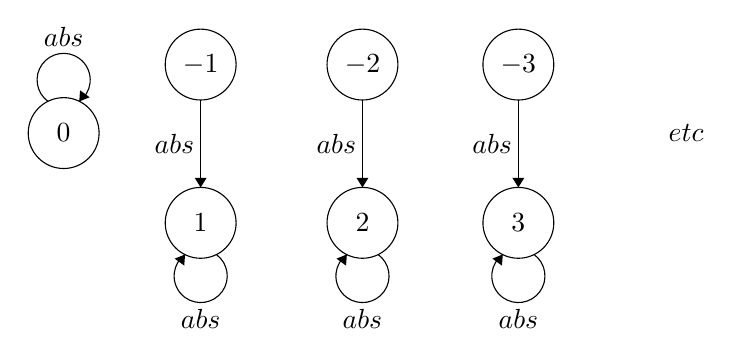
\begin{tikzpicture}[scale=0.15]
\tikzstyle{every node}+=[inner sep=0pt]
\draw [black] (14.4,-29.1) circle (3);
\draw (14.4,-29.1) node {$0$};
\draw [black] (26,-23.3) circle (3);
\draw (26,-23.3) node {$-1$};
\draw [black] (26,-36.7) circle (3);
\draw (26,-36.7) node {$1$};
\draw [black] (39.7,-23.3) circle (3);
\draw (39.7,-23.3) node {$-2$};
\draw [black] (39.7,-36.7) circle (3);
\draw (39.7,-36.7) node {$2$};
\draw [black] (52.9,-23.3) circle (3);
\draw (52.9,-23.3) node {$-3$};
\draw [black] (52.9,-36.7) circle (3);
\draw (52.9,-36.7) node {$3$};
% \draw [black] (67.1,-29.1) circle (3);
\node at (67.1,-29.1) {$etc$};
\draw [black] (13.077,-26.42) arc (234:-54:2.25);
\draw (14.4,-21.85) node [above] {$abs$};
\fill [black] (15.72,-26.42) -- (16.6,-26.07) -- (15.79,-25.48);
\draw [black] (26,-26.3) -- (26,-33.7);
\fill [black] (26,-33.7) -- (26.5,-32.9) -- (25.5,-32.9);
\draw (25.5,-30) node [left] {$abs$};
\draw [black] (27.323,-39.38) arc (54:-234:2.25);
\draw (26,-43.95) node [below] {$abs$};
\fill [black] (24.68,-39.38) -- (23.8,-39.73) -- (24.61,-40.32);
\draw [black] (39.7,-26.3) -- (39.7,-33.7);
\fill [black] (39.7,-33.7) -- (40.2,-32.9) -- (39.2,-32.9);
\draw (39.2,-30) node [left] {$abs$};
\draw [black] (41.023,-39.38) arc (54:-234:2.25);
\draw (39.7,-43.95) node [below] {$abs$};
\fill [black] (38.38,-39.38) -- (37.5,-39.73) -- (38.31,-40.32);
\draw [black] (54.223,-39.38) arc (54:-234:2.25);
\draw (52.9,-43.95) node [below] {$abs$};
\fill [black] (51.58,-39.38) -- (50.7,-39.73) -- (51.51,-40.32);
\draw [black] (52.9,-26.3) -- (52.9,-33.7);
\fill [black] (52.9,-33.7) -- (53.4,-32.9) -- (52.4,-32.9);
\draw (52.4,-30) node [left] {$abs$};
\end{tikzpicture}
\end{center}


Every permutation $g$ of $\mathbb{Z}^+$ can be extended to an automorphism $h$ of $A$ by setting $h(i)=g(i)$, for $i\in \mathbb{Z}^+$; $h(0)=0$; and $h(i)=-g(-i)$, for $i<0$. 

\begin{aside}
    Why is this? The only relation we have in our graph is the absolute-value relation, so our graph looks like a bunch of pairs $n, -n$ (for $n$ positive) where there is an edge from $-n$ to $n$ and an edge from $n$ to $n$ (ie a self-loop at $n$), plus $0$ all on its own with a self-loop. So long as we keep $0$ fixed in place, permuting any of our $(n, -n)$-pairs gives us an automorphism, provided that we match don't ``flip'' any of the pairs - ie, negative numbers (which have in-degree 0) map to negative numbers, and positive numbers (which have in-degree 2) map to positive numbers. The formulae mentioned above ensure that this happens. 
\end{aside}



Let's write $\mathbb{Z}^-$ for the set of negative integers. Thus, $\autorbs{A}= \{\mathbb{Z}^+,\{0\},\mathbb{Z}^-\}$. Each orbit of $\aut{A}$ acting on $U^A$ is definable:
\begin{itemize}
\item 
$S_1[A] = \mathbb{Z}^+$, where $S_1(x)$ is $(\exists y)(y\neq x \wedge Lyx)$;
\item 
$S_2[A] = \mathbb{Z}^-$, where $S_2(x)$ is $(\forall y)\neg Lyx$;
\item 
$S_3[A] = \{0\}$, where $S_3(x)$ is $\neg S_1(x)\wedge\neg S_2(x)$.
\end{itemize} 

\begin{aside}
    $S_1[A] = \mathbb{Z}^+$ as the positive integers are the only ones which have in-neighbours distinct from themselves (because there is an edge from a negative integer to its positive absolute value). Explain in your own words why $S_2[A] = \mathbb{Z}^-$ and $S_3[A] = \{0\}$. 
\end{aside}

By Corollary \ref{def-orbs-cor}, it follows that there are exactly eight sets definable in $A$:
\begin{enumerate}
\item $\emptyset$,
\item $\{0\}$,
\item $\mathbb{Z}^+$,
\item $\mathbb{Z}^-$,
\item $\mathbb{Z}^+\cup\mathbb{Z}^-$,
\item $\mathbb{Z}^+\cup\{0\}$,
\item $\mathbb{Z}^-\cup\{0\}$,
\item $\mathbb{Z}$.
\end{enumerate}

\subsubsection*{Defining Infinite Graphs Themselves}
We've just figured out which subsets of $A$ are definable, but what about $A$ itself - ie, can $A$ be uniquely specified by some schema?

The situation would be simpler if we had a finite graph.
\begin{theorem}
If $D$ is a finite graph, then there is a schema $S$ such that for every graph $D'$, 
\[
D'\models S \mbox{ if and only if } D'\cong D.
\]
\end{theorem}

\begin{aside}
    Give a proof of this theorem. Intuitively, the idea is that if a graph is finite, you only need to specify finitely many things about it (eg how many nodes there are, which nodes are connected by edges) in order to uniquely pick out the graph. 
\end{aside}

In sharp contrast, the following theorem shows that \emph{no} infinite structure can be perfectly described by any schema. In order to state the result, we need to define $\theo{D}$, the \emph{complete theory of} $D$:
\[
\theo{D} = \{S\mid S \mbox{ is a schema and } D\models S\}. 
\]
\begin{theorem}\label{infnotcat-thm}
For every infinite graph $D$, there is a graph $D'$, $D'\models\theo{D}$ and $D'\not\cong D$.
\end{theorem}
Theorem \ref{infnotcat-thm} is a corollary to the Compactness Theorem for PQT, a fundamental\footnote{By many accounts, this is \emph{the} most fundamental result about First-Order Logic (the common name for what we call PQT).} result we will study shortly.

\subsubsection*{A Rigid Structure: The Natural Numbers with Successor}
We now look at another infinite structure $B$ where definability behaves very differently. $B$ is described by:
\[
    U^B = \mathbb{N}, L^B = \{\op{i}{j}\mid j=i+1\}
\]

\begin{center}
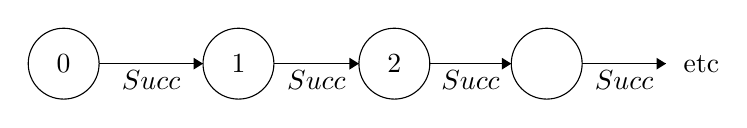
\begin{tikzpicture}[scale=0.15]
\tikzstyle{every node}+=[inner sep=0pt]
\draw [black] (12,-29.5) circle (3);
\draw (12,-29.5) node {$0$};
\draw [black] (26.8,-29.5) circle (3);
\draw (26.8,-29.5) node {$1$};
\draw [black] (40,-29.5) circle (3);
\draw (40,-29.5) node {$2$};
\draw [black] (52.9,-29.5) circle (3);
% \draw (52.9,-29.5) node {$3$};
\node at (66,-29.5) {etc};
\draw [black] (15,-29.5) -- (23.8,-29.5);
\fill [black] (23.8,-29.5) -- (23,-29) -- (23,-30);
\draw (19.4,-30) node [below] {$Succ$};
\draw [black] (29.8,-29.5) -- (37,-29.5);
\fill [black] (37,-29.5) -- (36.2,-29) -- (36.2,-30);
\draw (33.4,-30) node [below] {$Succ$};
\draw [black] (43,-29.5) -- (49.9,-29.5);
\fill [black] (49.9,-29.5) -- (49.1,-29) -- (49.1,-30);
\draw (46.45,-30) node [below] {$Succ$};
\draw [black] (55.9,-29.5) -- (63,-29.5);
\fill [black] (63,-29.5) -- (62.2,-29) -- (62.2,-30);
\draw (59.45,-30) node [below] {$Succ$};
\end{tikzpicture}
\end{center}

A first observation is that $\aut{B}=\{e\}$, that is, $B$ is a rigid structure. Intuitively, any homomorphism must map $0$ to itself, since it is the only element which doesn't have anything less than it. Similary, any homomorphism must map any positive $n$ to itself, since $n$ is the only number with exactly $n - 1$ predecessors. 

We can establish this formally by mathematical induction. Suppose $h$ is an automorphism of $B$. Since $0$ is the only node of $B$ with in-degree $0$, we must have $h(0)=0$. Now suppose, as induction hypothesis, that $h(n)=n$. Since $n+1$ is the only member of $U^B$ to which $n$ is related, it follows from the hypothesis that $h$ is an automorphism that $h(n+1)=n+1$. It follows that for all $k\in U^B$, $h(k)=k$. Hence, $\aut{B}=\{e\}$. 

This argument suggests that for every $k\in U^B$, $\{k\}$ is definable over $B$. Let's show this, again by induction. First, the schema $S^0(x): (\forall y)\neg Lyx$ defines $\{0\}$ over $B$. Next, as induction hypothesis, suppose that $S^n(x)$ defines $\{n\}$ over $B$. Let $z$ be a variable which does not occur anywhere in $S^n(x)$ and let $S^n(z)$ be the result of replacing $x$ with $z$ at all its occurrences in $S^n(x)$. Then the schema $(\exists z)(S^n(z)\wedge Lzx)$ defines $\{n+1\}$ over $B$. this completes the induction and establishes that for every $k\in U^B$, $\{k\}$ is definable over $B$. It follows at once that every finite subset of $U^B$ and every co-finite subset of $U^B$ is definable over $B$. 

\begin{aside}
    Why is it important that $z$ be a variable which occurs nowhere in $S^n(x)$?
\end{aside}

What other subsets of $U^B$ are definable over $B$? Note that since $B$ is rigid, there is no possibility of exhibiting an automorphism $h$ of $B$ with $h[X]\neq X$, that is, the ``automorphism method'' is powerless to establish the undefinability of any subset of $U^B$ in $B$. Could it be that every subset of $U^B$ is definable over $B$? 




\newpage

\subsection{Undefinability}
\subsubsection*{Cantor's Theorem and Cardinality Arguments}
We will show that for every infinite structure $C$ there is a subset $X\subseteq U^C$ which is \emph{not} definable over $C$. This result is a corollary to the celebrated Cantor Diagonal Theorem.
\begin{theorem}[Cantor]\label{cantordiag-thm}
Let $U$ be an infinite set and let $V_1, V_2, \ldots$ be a sequence of subsets of $U$. There is subset $W$ of $U$ such that for all $i\geq 1$, $W\neq V_i$.
\end{theorem}
\emph{Proof}: Suppose $U$ is an infinite set. Let $U^*= \{a_1, a_2, \ldots\}$ be a countably infinite subset of $U$ and let $V_1, V_2, \ldots$ be a sequence of subsets of $U$. Let $W=\{i\mid a_i\not\in V_i\}$. Note that for every $i$, $a_i\in W$ if and only if $a_i\not\in V_i$. It follows that for all $i$, $W\neq V_i$. \qed

\begin{aside}
    The idea in the above proof is to show that, regardless of which way we list the subsets $V_i$ of $U$, there will always be some other subset $W$ of $U$ which is not in the list. We construct $W$ by making sure it differs from each $V_i$ by at least one element; to do this, it suffices to let $a_i \in W$ iff $a_i \not \in V_i$. 
\end{aside}

In order to apply Theorem \ref{cantordiag-thm} to questions about definable sets we require the following result.
\begin{theorem}\label{countschema-thm}
For every structure $C$, there is a sequence $V_1,V_2,\ldots$ of subsets of $U^C$ such that for every set $X$ definable over $C$, there is an $i$ such that $X=V_i$. 

For those who know a little bit of set theory, this says that there are only countably many definable subsets of any given structure.
\end{theorem}
\emph{Proof}: Every schema is a finite sequence of symbols drawn from a finite alphabet. Thus, we may arrange all schemata $S(x)$ in a list $S_1(x), S_2(x),\ldots$, first ordered by length, and then within length, alphabetically. We obtain a list $V_1,V_2,\ldots $ of all the sets definable over $C$ by setting $V_i=S_i[C]$ for all $i$. \qed

As Theorems \ref{cantordiag-thm} and Theorem \ref{countschema-thm} entails that we can list all definable subsets of an infinite structure $C$, and theorem \ref{cantordiag-thm} entails that no list can exhaust all the definable subsets of an infinite set. So we have our result:

\begin{corollary}
For every infinite structure $C$ there is a subset $X\subseteq U^C$ which is not definable over $C$.
\end{corollary}

\subsubsection*{The Compactness Theorem and Automorphisms of ``Non-standard Models''}

Of course, this gives us no idea which particular sets are not definable over a given infinite structure. In the case of the graph $B$ introduced above, we will show that if a set is neither finite nor co-finite, it is \emph{not} definable over $B$. In order to establish this, we will deploy one of the fundamental properties of polyadic quantification theory: \emph{compactness}. First, some definitions requisite to the Compactness Theorem for Polyadic Quantification Theory.

\begin{definition}
A schema $S$ is \emph{satisfiable} if and only if for some structure $A$, $A\models S$.
\end{definition}

\begin{definition}
A set of schemata $\Gamma$ is \emph{satisfiable} if and only if there is structure $A$ such that for every schema $S\in \Gamma$, $A\models S$.
\end{definition}

\begin{definition}
A set of schemata $\Gamma$ is \emph{finitely satisfiable} if and only if for every finite set $\Delta\subseteq\Gamma$, $\Delta$ is satisfiable.
\end{definition}

\begin{theorem}[Compactness Theorem]\label{compact-thm}
For every set $\Gamma$ of schemata  of polyadic quantification theory, if $\Gamma$ is finitely satisfiable, then $\Gamma$ is satisfiable. 
\end{theorem}

Though the Compactness Theorem makes no mention of the notion of a derivation, one of its well-known proofs proceeds via the elaboration of a sound and complete formal system for logical deduction. This development will occupy our attention for much of the remainder of the course. For the moment, let's see how we can apply the Compactness Theorem to complete the analysis of the definable subsets of the structure $B$ specified above.
\begin{theorem}
If $V\subseteq U^B$ is definable over $B$, then $V$ is finite or $V$ is co-finite.
\end{theorem}
\emph{Proof}:
Suppose toward a contradiction that a schema $\sigma(x)$ defines a set $V$ which is neither finite nor co-finite over $B$. Let $\Lambda = \{ S\mid B\models S\}$; $\Lambda$ is the set of all schemata true in the structure $B$ and is often called the \emph{complete theory} of $B$. Let $y$ and $z$ be fresh variables which occur nowhere in $\Lambda$, $\sigma(x)$, or any of the schemata $S^n(x)$ for $n\geq 0$ (recall that $S^n(x)$ says that $x$ is the $n^{th}$ successor of the unique element with no predecessors). 

Define the set of schemata $\Gamma$ as follows.
\[
\Gamma = \Lambda\cup\{y\neq z \land \sigma(y) \land \neg \sigma(z)\}\cup\{\neg S^n(y) \land \neg S^n(z)\mid n\geq 0\}.
\]

Let $\Delta$ be a finite subset of $\Gamma$. As both $\sigma[B]$ and $\neg \sigma[B]$ are infinite by hypothesis, $\Delta$ can be satisfied by $B$ with suitable assignments from $U^B$ to the variables $y$ and $z$. Hence, by the Compactness Theorem, $\Gamma$ itself is satisfiable. Of course, if the structure $C$ satisfies $\Gamma$, then $C$ is not isomorphic to $B$ since the the elements of $U^C$ assigned to $y$ and $z$ in $C$ (call them $a$ and $b$ respectively) are not reachable in $C$ from the unique element of $C$ with no predecessor (whereas every element $b \in B$ is reachable in this manner). 

We will show that there is an automorphism $h$ of $C$ with $h(a)=b$. This will yield the desired  contradiction, since $C\models \sigma(y|a)$ and $C\models \neg \sigma(z|b)$. 

Note that $B$, and hence $C$, satisfy the following schemata.
\begin{itemize}
\item
$(\exists x)(\forall y)((\forall z)\neg Lzy \equiv x=y)$
\item
$(\forall x)(\exists y)(\forall z)(Lxz\equiv z=y)$
\item
$(\forall x)(\forall y)(\forall z)((Lxz\wedge Lyz)\supset x=y)$
\item
$(\forall x)\neg Lxx\\
\vdots\\
(\forall x)(\forall y_1)\ldots(\forall y_n)\neg Lxy_1\wedge Ly_1y_2\ldots\wedge Ly_nx\\
\vdots$
\end{itemize} 
The first three schemata guarantee that $L^C$ is an injective functional relation which is ``almost'' surjective -- there is a unique element of $U^C$ which lacks a pre-image under the function whose graph is $L^C$. Note that this guarantees that $U^C$ is infinite. 

\begin{aside}
    Why does this ensure that $U^C$ is infinite?
\end{aside}

The final infinite list of schemata guarantee that the the function whose graph is $L^C$ contains no finite cycles. Since $C$ is not isomorphic to $B$, all this implies that $C$ consists of an $L^C$ chain that is isomorphic to $B$ and a non-empty set of $L^C$ chains each of which is isomorphic to $\mathbb{Z}$ (the set of all integers) equipped with its usual successor relation. But, since $a$ and $b$ must lie on one or two of these ``$\mathbb{Z}$-chains,'' there is an automorphism $h$ of $C$ with $h(a)=b$ (if they lie on a single $\mathbb{Z}$-chain, shifting the $\mathbb{Z}$-chain works as an automorphism, whereas if they lie on two $\mathbb{Z}$-chains, interchanging the $\mathbb{Z}$-chains suffices). \qed
\newpage

\subsection{Proof}\label{pqt-proof-subsec}
\subsection*{Philosophy}
Up to this point, we have focussed primarily on questions surrounding the expressive power of polyadic quantification: which classes of structures can be characterized by (sets of) schemata of polyadic quantification theory; which sets of numbers are the spectra of schemata; what subsets of the universe of discourse of a structure can be defined by schemata. We now leave expressivity and turn towards a study of implication in the context of polyadic quantification theory. 

As we saw before, the mechanical decidability of validity of schemata (over a fixed, effectively presented vocabulary of sentence letters)
in the case of truth-functional logic, follows immediately from 
the definition of validity, since there are only finitely many truth assignments to a finite collection of sentence letters, and since the truth-value of a schema under any such assignment can be mechanically (even efficiently) evaluated\footnote{Of course, it remains an open problem  -- the $P/NP$ problem -- whether validity itself can be decided efficiently.}. In the case of MQT, though there are infinitely many structures interpreting the vocabulary of a fixed schema $S$, by means of the Small Model Theorem we were able to establish that we could effectively determine from $S$ a finite collection of finite structures such that $S$ is valid if and only if satisfied by every structure in this collection. Again, the satisfaction relation itself is mechanically decidable for finite structures, and thus validity of monadic schemata is mechanically decidable.

When we come to polyadic quantification theory, the situation is dramatically different. We will later see that the set of valid schemata of polyadic quantification theory, even restricted to the language of directed graphs, is \emph{not} decidable (the Church-Turing Theorem), though it is \emph{semi-decidable} (the G\"{o}del Completeness Theorem; see Definition \ref{sem-dec-def} for a definition of semi-decidability). 

We will soon begin a detailed study of systematic techniques to establish that a schema of polyadic quantification theory is valid. For simplicity, we will again just consider schemata in the vocabulary with identity and a single dyadic predicate letter $L$ (the language of love, or directed graphs, as the less romantic are wont to say). Let's remind ourselves of the relevant definitions.
\begin{definition}
A schema $S$ is \emph{valid} if and only if for every structure $A$, $A\models S$. We write \val\ for the set of valid schemata (in the language of directed graphs). 
\end{definition}

\begin{definition}
A schema $S$ is \emph{finitely valid} if and only if for every structure $A$, with $U^A=[n]$, for some $n$, $A\models S$. We write \fval\ for the set of finitely valid schemata (in the language of directed graphs).
\end{definition}

If we think about what it means for a schema to be valid (ie, to be true in all models -- including arbitrarily large infinite models), there is no evident way to describe a procedure for determining if a schema is valid: there are too many structures, and for some infinite structures $A$ we may have no mechanical procedure to determine whether $A$ satisfies a given schema. Finite validity, or at least it's complement (finite invalidity), fares better. 

\subsubsection*{\fval\ is Semi-Decidable}
For any directed graph $A$ with universe $[n]$ and any schema $S$, we can mechanically decide whether $A\models S$. Moreover, we can design a procedure, call it $M$ to effectively enumerate all such graphs in a sequence $A_0, A_1, \ldots$ and successively test whether $A_i\models S$ for a given schema $S$. 

\begin{aside}
    When we say ``design a procedure'', what we mean formally is \emph{specify a Turing Machine}. A \emph{Turing Machine} is a simple model of computation which (all reasonable mathematicians and compter-scientists agree) completely captures the intuitive notion of ``computability''; that is, if something can be ``computed'' in the intuitive sense of being calculated by a sequence of mechanical actions, a suitably specified Turing Machine could compute it as ell, and vice-versa. 

    Turing Machines, along with other equivalent formulations of computation (eg the Lambda Calculus, Markov Algorithms, Partial Recursive Functions, etc), all act as a formal basis for our study of provability. If you are interested in Turing Machines or computation, CIS 262 is Penn's relevant introductory course. 
\end{aside}

If $S\not\in\fval$, then $M$ will eventually discover this, since in this case there is an $i$ such that $A_i\not\models S$. On the other hand, if $S\in\fval$, $M$ will run forever with input $S$ and we will get no information, ever waiting to see a non-existent counterexample to $S$. We say $M$ is a \emph{semi-decision procedure} for the complement of \fval:  given any schema $S$, $M$ correctly identifies $S$ as not finitely valid, if this is the case, and provides no information (the computation via $M$ \emph{diverges}) otherwise. 

\begin{definition}
    A \emph{semi-decision procedure} for a set $X$ is a mechanical procedure (eg a Turing Machine) which, when give input $A$, outputs ``TRUE'' within finite time if $A \in X$ and and runs indefinitely (eg, diverges) if $A \not \in X$.
\end{definition}

\begin{definition}\label{sem-dec-def}
    We say a set $X$ is \emph{semi-decidable} if there is a semi-decision procedure for $X$. 
\end{definition}

\begin{definition}
    A set $X$ is \emph{decidable} if there is a mechanical procedure (eg, Turing Machine) which, given input $A$, outputs ``TRUE'' in finite time if $A \in X$ and outputs ``FALSE'' in finite time if $A \not \in X$. 

    By the Church-Turing Thesis (the belief that Turing Machines adequately capture the intuitive notion of computation), this coincides with the informal notion of decidability we have used throughout the course. 
\end{definition}

Note what is critical here: there is a decidable relation on finite graphs $A$ and schemata $S$, namely the relation of satisfaction, and a means of effectively enumerating all finite graphs. We can think of a finite graph which falsifies a schema $S$ as a proof that $S$ is \emph{not} valid. That is, we can think of the procedure $M$ as a proof-search procedure for non-finite-validity. Note, if there were such a procedure $M^*$ for finite validity, then finite validity would be decidable.

\begin{aside}
    Why? Because with input a given schema $S$, we could execute the procedures $M$ and $M^*$ simultaneously with input $S$. One of the two is guaranteed to terminate and yield the correct answer. In general, if a set $X$ and its complement are both semi-decidable, then $X$ is decidable. 
\end{aside}


Let's return to consider \val. Again, the definition of \val\ suggests no semi-decision procedure for either \val\ or its complement. Already many times during the course we have presented arguments to establish the validity of one schema or another, or for various general statements about finite graphs, \emph{etc.} Such arguments ahve been informal, but, let us hope, rigorous. That is, they proceeded by means that established  that their conclusions were valid or were implied by their premisses. Of course, the arguments were not entirely explicit, so it was always legitimate to ask for one step or another to be elaborated to clarify its legitimacy. We might wonder: was the original argument a proof of its conclusion, or only the argument with the elaboration -- because if the original argument did not carry conviction, it wasn't a proof. Considerations of this sort lead in the direction of demanding ever higher standards for the explicitness of proofs and ultimately to the quest for formal proof. In the context of polyadic quantification theory, we may represent this as the quest for a system of deduction with a decidable proof relation, that is, a mechanically decidable relation $\ded{D}{S}$ which holds between a sequence of schemata $D$ and a schema $S$ if and only if $D$ is a deduction of $S$ via the rules of the system. We require that the system allow to deduce only valid schemata, that is, it should have the \emph{Soundness Property}: if there a deduction $D$ such that $\ded{D}{S}$, then $S\in\val$. Moreover, it would be desirable if our system would allow us to deduce every valid schema, that is, that it would have the \emph{Completeness Property}: if $S\in\val$, then there is a deduction $D$ such that $\ded{D}{S}$. 

\begin{definition}
    A proof-system is \emph{sound} if every provable sentence is valid. Schematically:
    \[
        (\exists D)(\ded{D}{S}) \text{ implies } S \in \val
    \]
\end{definition}

\begin{definition}
    A proof-system is \emph{complete} is every valid sentence is provable. Schematically:
    \[
        S \in \val \text{ implies } (\exists D)(\ded{D}{S})
    \]
\end{definition}

\subsubsection*{History and Epistemology of Proof}
The elaboration of formal systems of deduction for polyadic quantification caps a long effort to achieve the highest possible degree of rigor in mathematical argumentation. This search was in part motivated by the periodic appearance of contradictions in the mathematical theory of the continuum (the real numbers). This theory, whose genesis may be dated to the Pythagoreans' proof that the square root of two is irrational, was developed with great vigor in the seventeenth century, in connection with the rise of the new physics and its effort to provide a unified theory of the motion of both terrestrial and celestial bodies. As mathematical analysis (as the theory of the continuum came to be called) developed in the nineteenth century, and became ever more enmeshed with new areas of physics, such as the theory of heat, the need for a more rigorous foundation for the subject became ever more pressing. In particular, even the greatest of mathematicians, such as Augustin Cauchy, were hampered by the lack of a perspicuous notation for iterated quantification in formulating suitable convergence conditions guaranteeing continuity for the limits of sequences of functions. Throughout the nineteenth century several mathematicians, among them Bernard Bolzano, Georg Cantor, Cauchy, and Richard Dedekind, strove to place the subject of analysis on a firm footing by reducing the the theory of the continuum to the theory of the integers (arithmetic) through the use of sets or sequences of rational numbers; the outcome of these efforts came to be known as ``the arithmetization of analysis'' and was celebrated by David Hilbert in his famous 1900 address to the International Congress of Mathematicians held in Paris as one of the great achievements of nineteenth-century mathematics. Late in the century, Gottlob Frege sought an even greater economy in the basic principles required for the rigorous foundation of analysis through his attempt to reduce arithmetic to logic. Though this effort was ultimately doomed by Russell's paradox, Frege's articulation of a calculus for logical deduction was a signal achievement in the development of modern logic. In reaction to the paradoxes, Hilbert, in collaboration with various of his students, and a number of other mathematicians, developed \emph{formal systems} of logic of the sort expounded in contemporary treatments deductive logic such as Goldfarb's text. 

From an epistemological point of view, one might insist that a mathematical proof should be self-certifying, that is, if the derivation \der{D}\ is a proof of the mathematical statement \stat{S}, then this should be immediately recognizable -- no further argument should be required to convince someone of this, for otherwise, it is not \der{D}\ itself, but only \der{D}\ supplemented with this additional argument, that constitutes a proof of \stat{s}. The notion of formal system takes this insistence to a natural limit: in a formal system the relation ``\der{D}\ is a proof of \stat{S}'' is mechanically decidable, that is, there is an algorithm which can be applied to the pair $\op{\der{D}}{\stat{S}}$ to determine whether the proof relation obtains. In a formal system of deduction $\forms{F}$ a derivation \der{D} consists of a finite sequence of schemata, and a statement \stat{S} is represented by a schema $S$. We write $\Pi_{\forms{F}}(\der{D},S)$ for ``\der{S}\ is a proof of $S$ in the formal system \forms{F}.'' The schema $S$ is a theorem of \forms{F}\ if and only if there is a derivation \der{d}\ such that $\Pi_{\forms{F}}(\der{D},S)$. We write $\vdash_{\forms{F}}S$ for ``S is a theorem of \forms{F}.'' In like fashion, we write $X\vdash_{\forms{F}}S$ for ``S is derivable from hypotheses $X$ in \forms{F}.''




\subsection*{Our Proof System}
We will use the proof-system for PQT which is described in detail on pages 181-216 of Warren Goldfarb's \emph{Deductive Logic}, often called \emph{natural deduction}. The qualifier ``natural'' is meant to indicate that we are able to reason relatively naturally within this formal system; in particular, natural deduction allows us to make arguments of the form
\begin{enumerate}
     \item Suppose $A$
     \item Hence $B$
     \item Therefore, if $A$, then $B$
\end{enumerate} 
This pattern involves introducing a new premise in step (1), inferring something from it in step (2), and then \emph{discharging} the premise in step (3). The ability to introduce and then discharge premises distinguished natural deduction from other systems of deduction which often require longer proofs. 

When we work out a deduction, we will do some bookkeeping in order to keep track of which premises we use at each stage, as well as which \emph{rules of inference} are being used. As such, the form of our deductions will be as follows: 
\begin{enumerate}
    \item Each line in a deduction will be numbered, beginning at (1)
    \item To the right of each line number will be the current schema under consideration
    \item To the left of each line number, there will be a set indicating the line numbers of premises upon which the current schema depends
    \item To the right of each schema we will place an acronym indicating which rule was used to arrive at the current schema, as well as the line number of the schema which that rule acted on. 
\end{enumerate}

For example, the following line would indicate that: this is the $4^{th}$ line of a deduction which depends on a premise from line $3$, the current schema is $(\exists y) Lwy$, and was derived from line $(3)$ by means of the rule \emph{Universal Instantiation}
\[
   \begin{array}{lll}
\{3\} & (4)\ (\exists y) Lwy & (3)\ \mathrm{UI}
\end{array} 
\]

\subsubsection*{Asymmetric implies Irreflexive}
We refer the reader to Goldfarb for an explanation of each of the rules of inference. Here, we present various deductions and explanations as example. First, a deduction using the rules described on pages 183 -- 185 of the text which shows that if a relation is asymmetric, then it is irreflexive.
\begin{center}
$\{(\forall x)(\forall y)(Lxy\supset\neg Lyx)\}$ implies $(\forall x)\neg Lxx.$
\end{center}
\[
\begin{array}{lll}
\{1\}   & (1)\  (\forall x)(\forall y)(Lxy\supset\neg Lyx) &  \mathrm{P}\\
\{1\}   & (2)\ (\forall y)(Lxy\supset\neg Lyx) & (1) \ \mathrm{UI}\\
\{1\}   & (3)\ Lxx\supset\neg Lxx &  (2)\ \mathrm{UI}\\
\{1\}   & (4)\ \neg Lxx   & (3)\ \mathrm{TF}\\
\{1\}   & (5)\ (\forall x) \neg Lxx  & (4)\ \mathrm{UG}
\end{array}
\]

\begin{aside}
    We first introduce the premise $(\forall x)(\forall y)(Lxy\supset\neg Lyx)$ (ie, we assume asymmetry), then universally instantiate twice to strip off the universal quantifiers (and thereby achieve a truth-functional schema). We can then make the truth-functional deduction $Lxx\supset\neg Lxx$ \emph{truth-functionally implies} $\lnot Lxx$. Lastly, we universally generalize to get the intended result. 
\end{aside}

\subsubsection*{Transitive and Irreflexive implies Asymmetric}
We show that if a relation is transitive and irreflexive, then it's asymmetric.
\begin{center}
$\{(\forall x)(\forall y)(\forall z)(Lxy\supset(Lyz\supset Lxz)), (\forall x)\neg Lxx\}$ implies $(\forall x)(\forall y)(Lxy\supset\neg Lyx).$
\end{center}
\[
\begin{array}{lll}
\{1\}   & (1)\  (\forall x)(\forall y)(\forall z)(Lxy\supset(Lyz\supset Lxz)) &  \mathrm{P}\\
\{1\}   & (2)\ (\forall y)(\forall z)(Lxy\supset(Lyz\supset Lxz)) & (1) \ \mathrm{UI}\\
\{1\}   & (3)\ (\forall z)(Lxy\supset(Lyz\supset Lxz)) &  (2)\ \mathrm{UI}\\
\{1\}   & (4)\ Lxy\supset(Lyx\supset Lxx)   & (3)\ \mathrm{UI}\\
\{5\}   & (5)\ (\forall x) \neg Lxx  & \ \mathrm{P}\\
\{5\}   & (6)\ \neg Lxx  & (5)\ \mathrm{UI}\\
\{1,5\}   & (7)\ (Lxy\supset\neg Lyx)  & (4,6)\ \mathrm{TF}\\
\{1,5\}   & (8)\ (\forall y)(Lxy\supset\neg Lyx)  & (7)\ \mathrm{UG}\\
\{1,5\}   & (9)\ (\forall x)(\forall y)(Lxy\supset\neg Lyx)  & (8)\ \mathrm{UG}
\end{array}
\]

\begin{aside}
    On line (1), we introduce a premise for transitivity. Lines 2-4 strip off the universal quantifiers to get the truth-functional part of the transitivity schema. Line (5) introduces a premise for irreflexivity, line (6) strips off its quantifier. Line (7) is a truth-functional inference from lines (4) and (6), an then lines (8, 9) reintroduce the universal quantifiers to achieve the intended result. 
\end{aside}

\subsubsection*{Argument by Cases}
Here is an example which illustrates the use of ``argument by cases'', which is used when we wish to show that a disjunction $A \vee B$ implies some schema $S$. To argue by cases, we show that $A$ implies $S$ and $B$ implies $S$, then truth-functionally infer that $A \vee B$ implies $S$. 

\begin{center}
$\{(\forall x)Fx\vee(\forall x)Gx\}$ implies $(\forall x)(Fx\vee Gx).$
\end{center}
\[
\begin{array}{lll}
\{1\}   & (1)\  (\forall x)Fx\vee(\forall x)Gx &  \mathrm{P}\\
\{2\}   & (2)\ (\forall x)Fx &  \ \mathrm{P}\\
\{2\}   & (3)\ Fx &  (2)\ \mathrm{UI}\\
\{2\}   & (4)\ Fx\vee Gx   & (3)\ \mathrm{TF}\\
\{2\}   & (5)\ (\forall x) (Fx\vee Gx)  & (4)\ \mathrm{UG}\\
\{\}   & (6)\ (\forall x)Fx\supset(\forall x) (Fx\vee Gx)   & \{2\}(5)\ \mathrm{D}\\
\{7\}   & (7)\ (\forall x)Gx &  \ \mathrm{P}\\
\{7\}   & (8)\ Gx &  (7)\ \mathrm{UI}\\
\{7\}   & (9)\ Fx\vee Gx   & (8)\ \mathrm{TF}\\
\{7\}   & (10)\ (\forall x) (Fx\vee Gx)  & (9)\ \mathrm{UG}\\
\{\}   & (11)\ (\forall x)Gx\supset(\forall x) (Fx\vee Gx)   & \{7\}(10)\ \mathrm{D}\\
\{1\}   & (12)\ (\forall x) (Fx\vee Gx)  & (1,6,11)\ \mathrm{TF}\\
\end{array}
\]

\begin{aside}
    Line (1) introduces our main premise. Line (2) introduces our first case, and line (3) universally instantiates it. Line (4) is a truth-functional inference from line (3), and line (5) universally generalizes line (4) in order to prepare for line (6), which discharges our premise from line 2 to show that the implication holds in the first case. Lines (7 - 11) play the same role for the second case as lines (2 - 6) did for the first case. Line (11) is a truth-functional inference from the two implications we just proved, and gives the intended result. 
\end{aside}


\subsubsection*{Quantifier Conversion (DeMorgan's Laws)}
We give a pair of deductions that legitimate the ``conversion of quantifiers rule'' which allows passing directly from $\neg(\forall x)S$ to $(\exists x)\neg S$ and \emph{vice versa}. These quantifier-conversion rules are often called \emph{DeMorgan's Laws}.
\begin{center}
$\{\neg(\forall x)Fx\}$ implies $(\exists x)\neg Fx.$
\end{center}
\[
\begin{array}{lll}
\{1\}   & (1)\  \neg(\forall x)Fx &  \mathrm{P}\\
\{2\}   & (2)\ \neg(\exists x)\neg Fx & (1) \ \mathrm{P}\\
\{2\}   & (3)\ (\forall x)\neg\neg Fx &  (2)\ \mathrm{CQ}\\
\{2\}   & (4)\ \neg\neg Fx   & (3)\ \mathrm{UI}\\
\{2\}   & (5)\ Fx   & (4)\ \mathrm{TF}\\
\{2\}   & (6)\ (\forall x)Fx  & (5)\ \mathrm{UG}\\
\{1,2\}   & (7)\ (\forall x)Fx\wedge\neg(\forall x)Fx  & (6)\ \mathrm{TF}\\
\{1\}   & (8)\ \neg(\exists x)\neg Fx\supset((\forall x)Fx\wedge\neg(\forall x)Fx)  & \{2\}(7)\ \mathrm{D}\\
\{1\}   & (9)\ (\exists x)\neg Fx  & (8)\ \mathrm{TF}
\end{array}
\]
\begin{center}
$\{(\exists x)\neg Fx\}$ implies $\neg(\forall x)Fx.$
\end{center}
\[
\begin{array}{lll}
\{1\}   & (1)\  (\forall x)Fx &  \mathrm{P}\\
\{2\}   & (2)\ (\exists x)\neg Fx & (1) \ \mathrm{P}\\
\{1\}   & (3)\ Fx &  (1)\ \mathrm{UI}\\
\{1\}   & (4)\ \neg\neg Fx   & (3)\ \mathrm{TF}\\
\{1\}   & (5)\ (\forall x)\neg\neg Fx   & (4)\ \mathrm{UG}\\
\{1\}   & (6)\ \neg(\exists x)\neg Fx  & (5)\ \mathrm{CQ}\\
\{1,2\}   & (7)\ \neg(\exists x)\neg Fx\wedge(\exists x)\neg Fx  & (6)\ \mathrm{TF}\\
\{2\}   & (8)\ (\forall x)Fx\supset(\neg(\exists x)\neg Fx\wedge(\exists x)\neg Fx)  & \{1\}(7)\ \mathrm{D}\\
\{1\}   & (9)\ \neg(\forall x)Fx  & (8)\ \mathrm{TF}
\end{array}
\]

\subsubsection*{Reductio ad Absurdum}

Here is an example of argument by \emph{reductio ad absurdum}, that, in addition, illustrates the use of the ``conversion of quantifiers'' rule we just deduced.  
\begin{center}
$(\exists y)(Py \supset (\forall x)Px)$ is valid
\end{center}
\[
\begin{array}{lll}
\{1\}   & (1)\ \neg (\exists y)(Py \supset (\forall x)Px)  & \mathrm{P}\\
\{1\}   & (2)\ (\forall y) \neg (Py \supset (\forall x)Px)  & (1)\
\mathrm{CQ}\\ 
\{1\}   & (3)\ \neg (Py \supset (\forall x)Px)  & (2)\ \mathrm{UI}\\
\{1\}   & (4)\ Py  & (3)\ \mathrm{TF}\\
\{1\}   & (5)\ (\forall x)Px  & (4)\ \mathrm{UG}\\
\{1\}   & (6)\ \neg (\forall x)Px \wedge (\forall x)Px  & (3)(5)\ \mathrm{TF}\\
\{\}   & (7)\ \neg (\exists y)(Py \supset (\forall x)Px) \supset & \{1\}(6)\
\mathrm{D}\\ 
  &\ \ \ \ (\neg (\forall x)Px \wedge (\forall x)Px) \\
\{\}   & (8)\ (\exists y)(Py \supset (\forall x)Px)  & (7)\ \mathrm{TF}
\end{array}
\]

Lines (1-7) derive a contradiction from the assumption the premise on line (1), which is the negation of what we intend to show. The intended result then follows by truth-functional implication. 

\subsubsection*{Existential Generalization and Instantiation}
The following gives an example of the use of existential generalization and instantiation, which allow us to  mirror common informal forms of argument involving the existential quantifier. 
\begin{center}
$\{(\forall x) ((\exists y) Lxy \supset (\forall z) Lzx), (\exists x)(\exists
y) Lxy \}$ implies $(\forall v)(\forall z) Lvz.$
\end{center}
\[
\begin{array}{lll}
\{1\}   & (1)\  (\exists x)(\exists y) Lxy &  \mathrm{P}\\
\{1,2\}   & (2)\ (\exists y) Lwy  & (1)w\ \mathrm{EII}\\
\{3\}   & (3)\ (\forall x) ((\exists y) Lxy \supset   & 
\mathrm{P}\\
  &\ \ \ \  (\forall z) Lzx)  & \\
\{3\}   & (4)\ (\exists y) Lwy \supset   & (3)\ \mathrm{UI}\\
  &\ \ \ \ (\forall z) Lzw & \\
\{1,2,3\}   & (5)\ (\forall z) Lzw  & (2)(4)\ \mathrm{TF}\\
\{1,2,3\}   & (6)\ Lvw  & (5)\ \mathrm{UI}\\
\{1,\not 2,3\}   & (7)\ (\exists y) Lvy  & (5)\ \mathrm{EG};\{2\}\
\mathrm{EIE}\\ 
\{3\}   & (8)\ (\exists y) Lvy \supset (\forall z) Lzv  & (3)\ \mathrm{UI}\\
\{1,3\}   & (9)\  (\forall z) Lzv & (7)(8)\ \mathrm{TF}\\
\{1,3\}   & (10)\  (\forall v)(\forall z) Lzv & (9)\ \mathrm{UG}
\end{array}
\]

When existentially instantiating, we replace a quantified variable (eg, $(\exists x)$) with a new constant (eg, $w$). It is important to instantiate using a new variable which does not occur elsewhere in the schema. 

\subsubsection*{Working With Identity}

Finally, we illustrate the use of the identity rules explained in Goldfarb. 
\begin{center}
$\{(\forall x) Rxx, \neg (\forall x)(\forall y) Rxy \}$
implies $\neg (\exists x)(\forall y) x = y$.
\end{center}
\[
\begin{array}{lll}
\{1\}   & (1)\ (\forall x) Rxx  & \mathrm{P}\\
\{2\}   & (2)\ \neg (\forall x)(\forall y) Rxy  & \mathrm{P}\\
\{3\}   & (3)\ (\exists x)(\forall y) x = y  & \mathrm{P}\\
\{3,4\}   & (4)\ (\forall y) u = y  & (3)u\ \mathrm{EII}\\
\{1\}   & (5)\ Ruu  & (1)\ \mathrm{UI}\\
\{3,4\}   & (6)\ u=y  & (4)\ \mathrm{UI}\\
\{\}   & (7)\ u=y \supset (Ruu \equiv Ruy) & \mathrm{III}\\
\{3,4\}   & (8)\ u=x  & (4)\ \mathrm{UI}\\
\{\}   & (9)\ u=x \supset (Ruy \equiv Rxy) & \mathrm{III}\\
\{1,3,   & (10)\ Rxy  & (5)(6)\ \mathrm{TF};\\
\not4\} &  & (7)(8)\ \{4\}\ \mathrm{EIE} \\
 & & (9)\\
\{1,3\}   & (11)\ (\forall y)Rxy  & (10)\ \mathrm{UG}\\
\{1,3\}   & (12)\ (\forall x)(\forall y)Rxy  & (11)\ \mathrm{UG}\\
\{1,2,3\}   & (13)\ p \wedge \neg p  & (2)(12)\ \mathrm{TF}\\
\{1,2\}   & (14)\ (\exists x)(\forall y) x = y  \supset
& \{3\}(13)\ \mathrm{D}\\
 & (p \wedge \neg p) & \\
\{1,2\}   & (15)\ \neg (\exists x)(\forall y) x = y  & (14)\ \mathrm{TF}
\end{array}
\]


\newpage

\subsection*{Showing Satisfiability}

Our last consideration will be the problem of establishing that a set of schemata $X$ is satisfiable. As we have noted, there is no uniform approach to this problem, since the collection of satisfiable schemata is \emph{not} semi-decidable. As such, showing satisfiability of a sentence $X$ amounts to constructing a structure $A$ such that $A \models X$. 

We give an example. Let $S$ be the conjunction of the following schemata.
\begin{itemize}
\item 
$(\forall x)(\forall y)(\forall z)((Lxy \wedge Lyz) \supset Lxz)$
\item
$(\forall x)(\forall y)(x\neq y\supset(Lxy \vee Lyx))$
\item
$(\forall x) \neg Lxx$
\item 
$(\forall x)((\exists y)Lxy\supset(\exists y)(Lxy\wedge (\forall z)\neg (Lxz\wedge Lzy)))$
\item 
$(\forall x)((\exists y)Lyx\supset(\exists y)(Lyx\wedge (\forall z)\neg (Lyz\wedge Lzx)))$
\item
$\neg(\forall x)(\exists y)Lyx$
\item
$\neg(\forall x)(\exists y)Lxy$
\end{itemize}
For each $n\geq 2$, let $R^n$ be the schema, 
\[
(\exists x_1)\ldots(\exists x_n)\bigwedge_{1\leq i< j\leq n}Lx_ix_j.
\]
Finally, let $X=\{S\}\cup\{R^n\mid n\geq 2\}$.

Is $X$ satisfiable? The first conjunct denotes transitivity, the second comparability, and the third irreflexivity, so we know we are working with a strict linear order. The fourth and fifth conjuncts say that successor and predecessor are both discrete. The sizth and seventh conjuncts say that there is a first and last element, respectively. The last set of schemata suffices to say that we must have infinitely many elements. 

At first, you may think that $X$ is not satisfiable - after all, a discrete linear order with endpoints certainly sounds like it must be finite. Intuition is often tricky when dealing with the infinite, though, so it's best to be careful. In fact, the union of the first seven schemata with any finite subset $\Delta$ of the set $\{R^n \mid n \geq 2\}$ is satisfiable - if $m$ is the largest integer for which $R^m$ appears in $\Delta$, a strict linear order of size $m$ suffices. So ever finite subset of $X$ is satisfiable, and hence by the Compactness Theorem, $X$ itself is satisfiable. 

Since $X$ is satisfiable, we must be able to construct some model for $A$ it. One such structure $A$ is defined as follows. 

\begin{itemize}
\item
$U^A=  \mathbb{Z}$.
\item
$L^A=\{\op{i}{j}\mid (0\leq i\mbox{ and } j<0)\mbox{ or }(i<j \mbox{ and }  (0\leq i,j\mbox{ or } i,j<0))\}$.
\end{itemize}

\begin{aside}
    Explain why $A \models X$. 
\end{aside}
\newpage

\subsection{Review}
\begin{mdframed}[linewidth=1]
\section*{Concept Review}
\textbf{Isomorphisms}: An \emph{isomorphism} is a function which preserves the structure of a model. Formally, an isomorphism from $A$ onto $B$ is a bijection $f$ from $U^A$ to $U^B$ such that $\langle f(i), f(j) \rangle \in L^B \iff \langle i, j \rangle \in L^A$. 

\textbf{Automorphisms}: An \emph{automorphism} an isomorphism from a structure $A$ onto itself; in other words, it is an isomorphism which leaves the edge-set unchanged. 

The \emph{automorphism class} of a structure is the set of all functions which are automorphisms on that structure. 

\textbf{Image of a Structure}: The \emph{image of a structure} $A$ under a function $f$ is the structure with same universe and edge relation defined by $L^{f[A]} := \{\langle f(i), f(j) \rangle \mid \langle i, j \rangle \in L^A\}$. 

\textbf{Orbit of a node}: The orbit of a node $a$ in a graph $A$ is the set of all possible images of that node under automorphisms of the graph. Intuitively, this is the set of all nodes which ``look the same, structurally'' as $a$. 

\textbf{Orbit of a graph}: The orbit of a graph $A$ of size $k$ under the action of $\symn{k}$ (the symmetry group of size $k$) is the maximal set of pairwise non-automorphic graphs which can be obtained from $A$ by actions in \symn{k}. In other words, this is the maximal set of graphs isomorphic to $A$, all with different edge-sets. 

\textbf{Definability in the Finite}: The only definable subsets of a finite graph are exactly the orbits of its nodes. We categorized all size-4 simple graphs and found all of their definable subsets. 

\textbf{Definability in the Infinite}: Every definable subset of an infinite graph is the orbit of some node. It is not the case (in general) that every orbit is definable, however, and so one must give an explicit schema which defines an orbit in order to assert that it is definable. We saw the examples of the integers with absolute-value and the natural numbers with successor. In the former case, we showed that there were $8$ possible definable sets, generated by the three orbits $\{0\}, \mathbb{Z}^{-}, \mathbb{Z}^{+}$. In the latter case, we used the Compactness Theorem to show that the only definable subsets were the finite and cofinite sets. 

\textbf{Orbit-Stabilizer Theorem}: We gave a proof for the Orbit-Stabilizer Theorem, which states that $|\symn{n}| = |\orb{A}{n}| \cdot |\aut{A}|$. 

\textbf{Proof}: We motivated the need for a formal system of proof, and showed that the set of finitely-valid sentences was \emph{semi-decidable}. We remarked that the set of valid sentences does not have an obvious semi-decision procedure like finite validity does, but that validity is still semi-decidable (!) because of the coinciding nature of truth and proof: the \emph{soundness} and \emph{completeness} theorems ensure that every valid formula is provable and vice-versa, and so by enumerating proofs we obtain a semi-decision procedure for validity. We remarked that non-validity (or equivalently, satisfiability) is not semi-decidable, because if it were then validity would itself be decidable (contradicting the Church-Turing Theorem). 

We gave examples of various proofs using the system of \emph{natural deduction} explained in Goldfarb. 
\end{mdframed}



\newpage
\begin{mdframed}[linewidth=1]
\section*{Problems}
\begin{enumerate}
    \item We say that a list $L$ of structures is \emph{succinct} iff no pair of structures on the list is isomorphic. Give a maximal succinct list of $\mod(S, 3)$ where 
    \[
        S := (\forall x)(\exists y)(\forall z)(Lxz \equiv z = y)
    \]

    \item For each structure $A$ in your list $L$ and each $O \in \autorbs{A}$, give a schema $S(x)$ such that $S[A] = O$. 

    \item Let $A$ be the structure with triadic predicate $P$ defined by 
    \[
        U^A = \mathbb{Z}, P^A = \{\langle i, j, k \rangle \mid |i - j| = k\}
    \]
    Is $X = \{i \in \mathbb{Z} \mid i < 0\}$ definable in $A$?

    \item Let $B$ be the structure with triadic predicte $Q$ defined by
    \[
        U^B = \mathbb{Z}, Q^B = \{\langle i, j, k \rangle \mid i + j = k\}
    \]
    Is $X = \{i \in \mathbb{Z} \mid i < 0\}$ definable in $B$?

    \item 
Let $X$ be the conjunction of the following schemata.
\begin{itemize}
\item 
$(\forall x)(\forall y)(\forall z)((Lxy \wedge Lyz) \supset Lxz)$
\item
$(\forall x)(\forall y)(x\neq y\supset(Lxy \vee Lyx))$
\item
$(\forall x) \neg Lxx$
\item 
$(\forall x)(\exists y)(Lxy\wedge (\forall z)\neg (Lxz\wedge Lzy))$
\item 
$(\forall x)(\exists y)(Lyx\wedge (\forall z)\neg (Lyz\wedge Lzx))$
\item
$(\forall x)(\exists y)(Lyx\wedge Fy)$
\item
$(\forall x)(\exists y)(Lxy\wedge Fy)$
\item
$(\forall x)(\forall y)((Fx\wedge Fy\wedge Lxy)\supset (\exists z)(Fz\wedge Lxz\wedge Lzy))$
\end{itemize}

Is $X$ satisfiable?
    
    \item Let 
    \[
        X = (\exists y)(\forall x)(Lxy \vee Lyx)
    \]
    \[
        S = (\forall x)(\exists y)(Lxy \vee Lyx)
    \]
    Does $X$ imply $S$? If so, give a deduction. If not, give a counterexample. 

    \item Let
    \[
        X = (\exists^{=5}x) \land (\forall x)(\lnot Lxx) \land (\forall xy)(Lxy \supset Lyx)
    \]
    \[
        S = (\exists xyz)(Lxy \land Lxz \land Lyz) \vee (\exists xyz)(\lnot Lxy \land \lnot Lxz \land \lnot Lyz)
    \]
    Does $X$ imply $S$? If so, give a deduction. If not, give a counterexample. 

    \item Let $S$ be the schema
    \[
            (\forall x)(Fx\supset(\exists y)(\neg Fy\wedge(\forall z)(Lxz\equiv y=z)))
    \]
    For each $n\geq 2$, let $R_n$ be the schema
    \[
    (\forall y)(\neg Fy\supset(\exists x_1)\ldots(\exists x_n)\bigwedge_{1\leq i<j\leq n}(x_i\neq x_j\wedge Fx_i\wedge Lx_iy));
    \]
    and for each $n\geq 2$, let $T_n$ be the schema
    \[
    (\exists x_1)\ldots(\exists x_n)\bigwedge_{1\leq i<j\leq n}(x_i\neq x_j\wedge \neg Fx_i).
    \]
    Let $X=\{S,R_n,T_n\mid n\geq 2\}$.

    Is $X$ satisfiable?

\end{enumerate}
\end{mdframed}

\newpage
\begin{mdframed}[linewidth=1]
\section*{Solutions}
\begin{enumerate}
    \item $S$ suffices to say that $L$ is a function. Drawing size-3 graphs leads us to the following maximal collection. 


    \begin{center}
    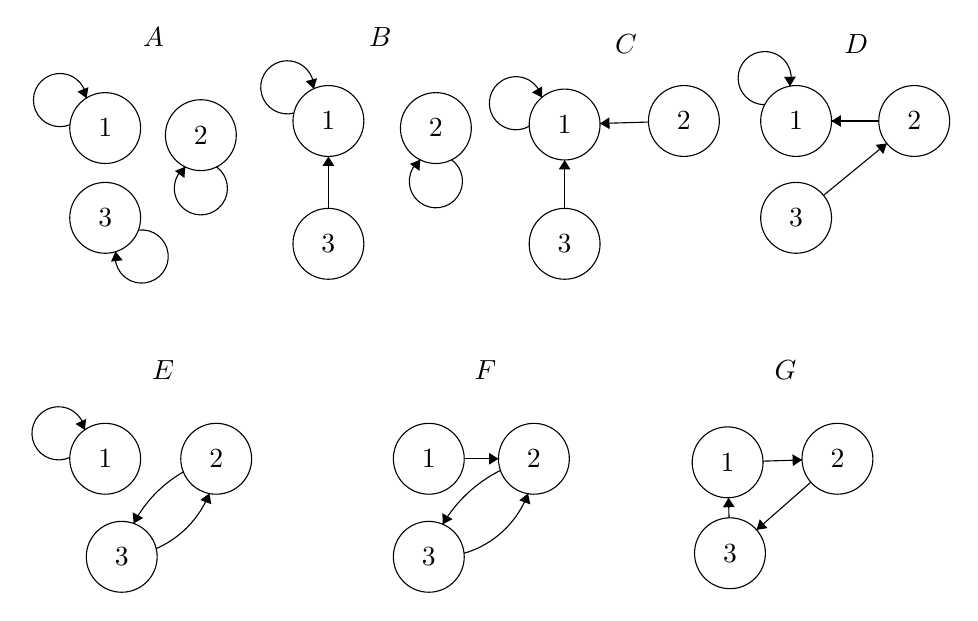
\begin{tikzpicture}[scale=0.15]
    \tikzstyle{every node}+=[inner sep=0pt]
    % \draw [black] (11.4,-11.3) circle (3);
    \draw (11.4,-11.3) node {$A$};
    % \draw [black] (30.6,-11.3) circle (3);
    \draw (30.6,-11.3) node {$B$};
    % \draw [black] (51.4,-11.9) circle (3);
    \draw (51.4,-11.9) node {$C$};
    % \draw [black] (70.9,-11.9) circle (3);
    \draw (70.9,-11.9) node {$D$};
    % \draw [black] (12.2,-39.5) circle (3);
    \draw (12.2,-39.5) node {$E$};
    % \draw [black] (39.5,-39.5) circle (3);
    \draw (39.5,-39.5) node {$F$};
    % \draw [black] (64.9,-39.5) circle (3);
    \draw (64.9,-39.5) node {$G$};
    \draw [black] (7.3,-19) circle (3);
    \draw (7.3,-19) node {$1$};
    \draw [black] (7.3,-26.6) circle (3);
    \draw (7.3,-26.6) node {$3$};
    \draw [black] (15.4,-19.6) circle (3);
    \draw (15.4,-19.6) node {$2$};
    \draw [black] (26.2,-18.4) circle (3);
    \draw (26.2,-18.4) node {$1$};
    \draw [black] (26.2,-28.8) circle (3);
    \draw (26.2,-28.8) node {$3$};
    \draw [black] (35.3,-19) circle (3);
    \draw (35.3,-19) node {$2$};
    \draw [black] (46.2,-18.7) circle (3);
    \draw (46.2,-18.7) node {$1$};
    \draw [black] (46.2,-28.8) circle (3);
    \draw (46.2,-28.8) node {$3$};
    \draw [black] (56.3,-18.4) circle (3);
    \draw (56.3,-18.4) node {$2$};
    \draw [black] (65.8,-18.4) circle (3);
    \draw (65.8,-18.4) node {$1$};
    \draw [black] (65.8,-26.6) circle (3);
    \draw (65.8,-26.6) node {$3$};
    \draw [black] (75.8,-18.4) circle (3);
    \draw (75.8,-18.4) node {$2$};
    \draw [black] (34.7,-47) circle (3);
    \draw (34.7,-47) node {$1$};
    \draw [black] (34.7,-55.3) circle (3);
    \draw (34.7,-55.3) node {$3$};
    \draw [black] (43.6,-47) circle (3);
    \draw (43.6,-47) node {$2$};
    \draw [black] (60,-47.3) circle (3);
    \draw (60,-47.3) node {$1$};
    \draw [black] (60.2,-55) circle (3);
    \draw (60.2,-55) node {$3$};
    \draw [black] (69.3,-47) circle (3);
    \draw (69.3,-47) node {$2$};
    \draw [black] (7.3,-47) circle (3);
    \draw (7.3,-47) node {$1$};
    \draw [black] (8.7,-55.3) circle (3);
    \draw (8.7,-55.3) node {$3$};
    \draw [black] (16.7,-47) circle (3);
    \draw (16.7,-47) node {$2$};
    \draw [black] (4.325,-18.714) arc (292.24052:4.24052:2.25);
    \fill [black] (5.72,-16.47) -- (5.88,-15.54) -- (4.95,-15.91);
    \draw [black] (10.101,-27.64) arc (97.36342:-190.63658:2.25);
    \fill [black] (8.18,-29.46) -- (7.79,-30.31) -- (8.78,-30.19);
    \draw [black] (16.723,-22.28) arc (54:-234:2.25);
    \fill [black] (14.08,-22.28) -- (13.2,-22.63) -- (14.01,-23.22);
    \draw [black] (26.2,-25.8) -- (26.2,-21.4);
    \fill [black] (26.2,-21.4) -- (25.7,-22.2) -- (26.7,-22.2);
    \draw [black] (23.289,-17.727) arc (284.71059:-3.28941:2.25);
    \fill [black] (24.96,-15.68) -- (25.24,-14.78) -- (24.28,-15.03);
    \draw [black] (36.623,-21.68) arc (54:-234:2.25);
    \fill [black] (33.98,-21.68) -- (33.1,-22.03) -- (33.91,-22.62);
    \draw [black] (46.2,-25.8) -- (46.2,-21.7);
    \fill [black] (46.2,-21.7) -- (45.7,-22.5) -- (46.7,-22.5);
    \draw [black] (43.215,-18.838) arc (300.37062:12.37062:2.25);
    \fill [black] (44.28,-16.41) -- (44.3,-15.47) -- (43.44,-15.98);
    \draw [black] (53.3,-18.49) -- (49.2,-18.61);
    \fill [black] (49.2,-18.61) -- (50.01,-19.09) -- (49.98,-18.09);
    \draw [black] (68.12,-24.7) -- (73.48,-20.3);
    \fill [black] (73.48,-20.3) -- (72.54,-20.42) -- (73.18,-21.2);
    \draw [black] (72.8,-18.4) -- (68.8,-18.4);
    \fill [black] (68.8,-18.4) -- (69.6,-18.9) -- (69.6,-17.9);
    \draw [black] (63.149,-17.021) arc (270.25384:-17.74616:2.25);
    \fill [black] (65.28,-15.46) -- (65.78,-14.65) -- (64.78,-14.66);
    \draw [black] (16.12,-49.927) arc (-21.35064:-66.54055:8.469);
    \fill [black] (16.12,-49.93) -- (15.36,-50.49) -- (16.29,-50.85);
    \draw [black] (9.706,-52.484) arc (152.38382:119.72499:10.806);
    \fill [black] (9.71,-52.48) -- (10.52,-52.01) -- (9.63,-51.54);
    \draw [black] (4.314,-46.878) arc (295.38954:7.38954:2.25);
    \fill [black] (5.58,-44.56) -- (5.69,-43.62) -- (4.79,-44.05);
    \draw [black] (43.101,-49.941) arc (-20.09413:-73.90163:8.208);
    \fill [black] (43.1,-49.94) -- (42.36,-50.52) -- (43.3,-50.86);
    \draw [black] (35.876,-52.549) arc (149.54048:116.46376:11.763);
    \fill [black] (35.88,-52.55) -- (36.71,-52.11) -- (35.85,-51.61);
    \draw [black] (37.7,-47) -- (40.6,-47);
    \fill [black] (40.6,-47) -- (39.8,-46.5) -- (39.8,-47.5);
    \draw [black] (67.05,-48.98) -- (62.45,-53.02);
    \fill [black] (62.45,-53.02) -- (63.38,-52.87) -- (62.72,-52.12);
    \draw [black] (60.12,-52) -- (60.08,-50.3);
    \fill [black] (60.08,-50.3) -- (59.6,-51.11) -- (60.6,-51.09);
    \draw [black] (63,-47.2) -- (66.3,-47.1);
    \fill [black] (66.3,-47.1) -- (65.49,-46.62) -- (65.52,-47.62);
    \end{tikzpicture}
    \end{center}

    \item Let $O_1 = \{1\}, O_2 = \{2\}, O_3 = \{3\}, O_4 = \{2, 3\}, O_5 = \{1, 2, 3\}$. Then 
    \begin{itemize}
        \item $\autorbs{A} = \{O_5\}$. This can be defined by the schema $(\forall x)(x = x)$. 

        \item $\autorbs{B} = \{O_1, O_2, O_3\}$. $O_1$ can be defined by $Lxx \land (\exists y)(Lyx \land y \neq x)$, $O_2$ can be defined by $Lxx \land \lnot (\exists y)(Lyx \land y \neq x)$, and $O_3$ can be defined by $\lnot Lxx$. 

        \item $\autorbs{C} = \{O_1, O_4\}$. $O_1$ can be defined by $Lxx$, and $O_4$ can be defined by $\lnot Lxx$. 

        \item $\autorbs{D} = \{O_1, O_2, O_3\}$. $O_1$ can be defined by $Lxx$, $O_2$ can be defined by $(\exists y)(Lyx \land x \neq y)$, and $O_3$ can be defined by $\lnot (\exists y)Lyx$. 

        \item $\autorbs{E} = \{O_1, O_4\}$. $O_1$ can be defined by $Lxx$, and $O_4$ can be defined by $\lnot Lxx$. 

        \item $\autorbs{F} = \{O_1, O_2, O_3\}$. $O_1$ can be defined by $\lnot (\exists y)Lyx$, $O_2$ can be defined by $(\exists yz)(Lyx \land Lxz \land z \neq y)$, and $O_3$ can be defined by $(\exists y)(\forall z)(Lzx \equiv y = z)$. 

        \item $\autorbs{G} = \{O_5\}$. This can be defined by the schema $(\forall x)(x = x)$. 
    \end{itemize}

    \item Yes, it is definable. $P^A$ is the \emph{distance relation}; $\langle i, j, k \rangle \in P^A$ iff the distance between $i, j$ is $k$. No two numbers have a negative distance, so we can define the set of all negative numbers by the schema
    \[
        (\forall yz)(\lnot Pyzx)
    \]

    \item No, it is not definable. The function $h$ defined by $h(i) = -i$ is an automorphism of $B$, but $h[X] \neq X$. 

    \item Yes, $X$ does imply $S$. Here is a derivation
    \[
\begin{array}{lll}
\{1\}   & (1)\ (\exists y)(\forall x)(Lxy \vee Lyx)  & \mathrm{P}\\
\{1, 2\} & (2)\ (\forall x)(Lxy \vee Lyx) & (1)y\ \mathrm{EII}\\
\{1, 2\} & (3)\ (Lxy \vee Lyx) & (2)\ \mathrm{UI}\\
\{1, 2\} & (4)\ (\exists y)(Lxy \vee Lyx) & (3)\ \mathrm{EG}\\
\{1\} & (5)\ (\exists y)(Lxy \vee Lyx) & (4)\{2\}\ \mathrm{EIE}\\
\{1\} & (6)\ (\forall x)(\exists y)(Lxy \vee Lyx) & (5)\ \mathrm{UG}
\end{array}
\]

    \item $X$ does not imply $S$. $X$ states that we have a simple graph of size 5, and $S$ expresses the \emph{three-mutuality} that we considered on day 1 of class. We shows that a ``friendship pentagon'' lacked 3-mutuality; that same pentagon acts as a counterexample here. 

    \item Yes, it is. To show this, we give a satisfying model for $X$. Recall that $\mathbb{Z}$ is the set of integers and $\mathbb{Q}^+$ is the set of positive rational numbers. Let $A$ be defined by
    \begin{itemize}
    \item
    $U^A= \mathbb{Q}^+\times\mathbb{Z}=\{\op{r}{i}\mid r\in\mathbb{Q}^+\mbox{ and}\ i\in \mathbb{Z}\}$ (the cartesian product of $\mathbb{Q}^+$ and $\mathbb{Z}$).
    \item
    $L^A=\{\op{\op{r}{i}}{\op{s}{j}}\mid r<s\}\cup\{\op{\op{r}{i}}{\op{s}{j}}\mid r=s\mbox{ and }i<j\}$.
    \end{itemize}

    Then $A \models X$. 

    \item Yes, it is. We show that $X$ is satisfiable by constructing a structure $B$ with $B\models X$. $B$ is defined by
    \begin{itemize}
    \item
    $U^B= \mathbb{Z}^+$.
    \item
    $F^B=\{2i\mid i\in\mathbb{Z}^+\}$.
    \item
    $L^B = \{\op{2^i\cdot j}{j}\mid i\in\mathbb{Z}^+\mbox{ and } j\not\in F^B\}$.
    \end{itemize}

\end{enumerate}
\end{mdframed}